\documentclass[14pt,a4paper]{extarticle}

% --- 1. Поддержка кириллицы, кодировок и шрифтов (СТП 01-2017) ---
\usepackage{cmap}
\usepackage[T2A]{fontenc}
\usepackage[utf8]{inputenc}
\usepackage[russian]{babel}
\usepackage{tempora} % Истинный Times New Roman для кириллицы и латиницы (с полной поддержкой Bold/Italic)
\usepackage{microtype}

% --- 2. Геометрия страницы по СТП 01-2017 и образцу ОтчетRest.docx (Левое 30мм, Правое 15мм, Верхнее 20мм, Нижнее 20мм) ---
\usepackage[a4paper, left=30mm, right=15mm, top=20mm, bottom=20mm]{geometry}

% --- 3. Межстрочный интервал (полуторный) и абзацный отступ (1.25 см) ---
\usepackage{setspace}
\setstretch{1.25}
\usepackage{indentfirst}
\setlength{\parindent}{1.25cm}
\setlength{\parskip}{0pt}

% --- 4. Предотвращение выезда длинных слов и идентификаторов за границы листа ---
\sloppy
\emergencystretch=2.5em
\righthyphenmin=2
\lefthyphenmin=2

% --- 5. Математические пакеты и таблицы ---
\usepackage{amsmath,amssymb}
\usepackage{array}
\usepackage{tabularx}
\usepackage{booktabs}
\usepackage{graphicx}
\usepackage{float}
\usepackage{caption}

% --- 6. Оформление подписей к рисункам и таблицам по СТП 01-2017 (длинное тире) ---
\DeclareCaptionLabelSeparator{emdash}{~---~}
\captionsetup[figure]{name=Рисунок, labelsep=emdash, justification=centering, font=normalfont, size=normalsize}
\captionsetup[table]{name=Таблица, labelsep=emdash, justification=raggedright, singlelinecheck=false, font=normalfont, size=normalsize}

% --- 7. Оформление заголовков разделов и подразделов по СТП 01-2017 (14pt, абзацный отступ 1.25 см) ---
\usepackage{titlesec}
\titleformat{\section}[block]{\bfseries\normalsize\raggedright}{\thesection}{1em}{\MakeUppercase}
\titleformat{\subsection}[block]{\bfseries\normalsize\raggedright}{\thesubsection}{1em}{}
\titleformat{\subsubsection}[block]{\bfseries\normalsize\raggedright}{\thesubsubsection}{1em}{}

\titlespacing*{\section}{\parindent}{18pt}{18pt}
\titlespacing*{\subsection}{\parindent}{18pt}{18pt}
\titlespacing*{\subsubsection}{\parindent}{18pt}{18pt}

% --- 8. Листинги кода по СТП 01-2017 (без номеров строк слева, с рамкой и переносом) ---
\usepackage{fvextra}
\usepackage{fancyvrb}
\DefineVerbatimEnvironment{CodeListing}{Verbatim}{
    fontsize=\fontsize{9.5pt}{11.5pt}\selectfont,
    framesep=2.5mm,
    framerule=0.5pt,
    breaklines=true,
    breakanywhere=true,
    breaksymbol={\tiny\ensuremath{\hookrightarrow}},
    xleftmargin=0pt,
    xrightmargin=0pt
}

% --- 9. Списки: отступы и стиль маркированных списков (маркер-тире как в CulinaryGuide) ---
\usepackage{enumitem}
\setlist{nosep, leftmargin=1.25cm}
\setlist[enumerate]{label=\arabic*., leftmargin=1.25cm}
\setlist[enumerate,1]{label=\arabic*., leftmargin=1.25cm}
\setlist[enumerate,2]{label=\arabic{enumi}.\arabic*., leftmargin=1.25cm}
\setlist[itemize]{label=-, leftmargin=1.25cm}
\renewcommand{\labelitemi}{-}
\renewcommand{\labelitemii}{-}

% --- 10. Нумерация страниц справа по СТП 01-2017 и образцу ОтчетRest.docx ---
\usepackage{fancyhdr}
\pagestyle{fancy}
\fancyhf{} % Очистка всех полей
\fancyfoot[R]{\thepage} % Номер страницы справа внизу
\renewcommand{\headrulewidth}{0pt}
\renewcommand{\footrulewidth}{0pt}

\fancypagestyle{plain}{
    \fancyhf{}
    \fancyfoot[R]{\thepage}
    \renewcommand{\headrulewidth}{0pt}
    \renewcommand{\footrulewidth}{0pt}
}

\begin{document}

% ==============================================================================
% ТИТУЛЬНЫЙ ЛИСТ (образцу ОтчетRest.docx и СТП 01-2017)
% ==============================================================================
\begin{titlepage}
    \begin{center}
        Министерство образования Республики Беларусь\\[0.15cm]
        Учреждение образования\\[0.15cm]
        «БЕЛОРУССКИЙ ГОСУДАРСТВЕННЫЙ УНИВЕРСИТЕТ\\
        ИНФОРМАТИКИ И РАДИОЭЛЕКТРОНИКИ»
    \end{center}
    
    \vspace{0.4cm}
    
    \begin{flushleft}
        Факультет компьютерных систем и сетей\\[0.1cm]
        Кафедра программного обеспечения информационных технологий\\[0.1cm]
        Дисциплина: Методы машинного обучения (ММО)
    \end{flushleft}
    
    \vspace{2.2cm}
    
    \begin{center}
        \large\textbf{ОТЧЕТ}\\[0.2cm]
        \normalsize
        {по лабораторной работе № 1}\\[0.3cm]
        Тема работы: Основы Python\\[0.2cm]
        Вариант № 2
    \end{center}
    
    \vspace{2.2cm}
    
    \noindent
    \begin{tabular}{@{}p{0.62\textwidth}@{}p{0.38\textwidth}@{}}
        Выполнила: & \\
        студентка гр. 351002 & Алексейчик Я.\,Н. \\[0.5cm]
        Проверил: & Лебедевич А.\,В.
    \end{tabular}
    
    \vfill
    
    \begin{center}
        Минск 2026
    \end{center}
\end{titlepage}

\setcounter{page}{2}

% ==============================================================================
% 1 ЦЕЛЬ ВЫПОЛНЕНИЯ РАБОТЫ
% ==============================================================================
\section{Цель выполнения лабораторной работы}

Целью выполнения лабораторной работы является комплексное освоение языка Python 3.12:
\begin{enumerate}
    \item \textbf{По части 1 (Базовые конструкции и структуры данных):} Изучение и практическое освоение синтаксических основ языка Python, динамической типизации, встроенных типов данных (числа, строки) и базовых коллекций (списки \texttt{list}, кортежи \texttt{tuple}, словари \texttt{dict}); реализация базовых математических алгоритмов (поиск простых чисел, фильтрация данных), обработка строковых последовательностей и создание интерактивного консольного интерфейса.
    \item \textbf{По части 2 (Функции, обработка исключений и матрицы):} Освоение принципов функциональной декомпозиции и процедурного программирования; приобретение навыков строгой статической типизации параметров функций (модуль \texttt{typing}); глубокое изучение и практическая реализация механизма структурной обработки исключительных ситуаций посредством блоков \texttt{try / except / else / finally}; разработка отказоустойчивых алгоритмов анализа вложенных двумерных числовых массивов.
    \item \textbf{По части 3 (Объектно-ориентированное программирование):} Практическое освоение парадигмы ООП в Python; проектирование пользовательских классов, реализация инкапсуляции, одиночного наследования и динамического полиморфизма; детальное разграничение статических атрибутов класса и динамических полей экземпляра; практическое применение методов экземпляра, фабричных методов класса (\texttt{@classmethod}) и утилитарных статических методов (\texttt{@staticmethod}).
\end{enumerate}

% ==============================================================================
% 2 КРАТКИЕ ТЕОРЕТИЧЕСКИЕ СВЕДЕНИЯ (до 4 страниц)
% ==============================================================================
\clearpage
\section{Краткие теоретические сведения}

\subsection{Базовый синтаксис языка Python и структуры данных}

Язык Python является высокоуровневым языком программирования с интерпретируемым выполнением инструкций и динамической строгой типизацией. Строгая типизация означает, что неявное преобразование несовместимых типов (например, сложение строки и числа \texttt{'10' + 5}) запрещено и вызывает ошибку \texttt{TypeError}. При этом динамическая природа языка позволяет одной переменной в разное время ссылаться на объекты различных типов.

\subsubsection{Фундаментальные структуры данных Python:}
\begin{itemize}
    \item \textbf{Списки (\texttt{list}):} Представляют собой изменяемые (\textit{mutable}) динамические массивы ссылок на объекты. Добавление элемента в конец списка методом \texttt{list.append()} выполняется за амортизированное время $O(1)$, вставка в произвольную позицию \texttt{list.insert()} требует сдвига элементов и занимает $O(n)$. Списки поддерживают списковые включения (\textit{list comprehensions}), позволяющие лаконично фильтровать и трансформировать коллекции:
    \begin{equation}
        L_{\text{нечет}} = [x \text{ for } x \in L \text{ if } x \bmod 2 \neq 0].
    \end{equation}
    \item \textbf{Кортежи (\texttt{tuple}):} Неизменяемые (\textit{immutable}) упорядоченные последовательности. После создания кортежа добавление, удаление или замена его элементов невозможны. Благодаря фиксированной длине кортеж аллоцируется единым компактным блоком памяти, что снижает накладные расходы по сравнению со списками. Кроме того, кортежи являются хешируемыми объектами (при условии, что все их элементы хешируемы), что позволяет использовать их в качестве ключей словарей и элементов множеств.
    \item \textbf{Словари (\texttt{dict}):} Ассоциативные структуры данных, реализованные на основе оптимизированных хеш-таблиц. Поиск, вставка и удаление элементов по ключу выполняются за среднее время $O(1)$. При обращении к словарю через метод \texttt{dict.get(key, default)} программа безопасно возвращает значение по умолчанию, если ключ отсутствует, не вызывая аварийного исключения \texttt{KeyError}.
\end{itemize}

В таблице~\ref{tab:structures_comp} приведено систематизированное сравнение встроенных коллекций Python.

\begin{table}[H]
    \centering
    \caption{Сравнительная характеристика основных структур данных Python}
    \label{tab:structures_comp}
    \small
    \begin{tabularx}{\textwidth}{|>{\raggedright\arraybackslash}p{2.4cm}|>{\raggedright\arraybackslash}p{2.2cm}|>{\centering\arraybackslash}p{2.2cm}|>{\centering\arraybackslash}p{2.2cm}|>{\raggedright\arraybackslash}X|}
        \hline
        \textbf{Структура} & \textbf{Синтаксис} & \textbf{Изменяе\-мость} & \textbf{Хешируе\-мость} & \textbf{Основная область применения} \\
        \hline
        Список (\texttt{list}) & \texttt{[1, 2, 3]} & Да & Нет & Динамические последовательности \\
        \hline
        Кортеж (\texttt{tuple}) & \texttt{(1, 2, 3)} & Нет & Да & Фиксированные наборы, ключи словарей \\
        \hline
        Словарь (\texttt{dict}) & \texttt{\{'k': 'v'\}} & Да & Нет & Ассоциативные таблицы, поиск $O(1)$ \\
        \hline
        Множество (\texttt{set}) & \texttt{\{1, 2, 3\}} & Да & Нет & Уникальные элементы, теория множеств \\
        \hline
    \end{tabularx}
\end{table}

\subsection{Функции и структурная обработка исключений}

Функции в Python объявляются с помощью ключевого слова \texttt{def} и представляют собой объекты первого класса (\textit{first-class citizens}) --- их можно передавать в качестве аргументов, сохранять в переменных и возвращать из других функций. Для предотвращения ошибок типизации используется модуль \texttt{typing} (аннотации \texttt{List}, \texttt{Tuple}, \texttt{Optional}, \texttt{Any}).

\textbf{Полный механизм обработки исключений (\texttt{try / except / else / finally}):}
\begin{itemize}
    \item \textbf{\texttt{try}:} В данный блок помещается программный код, при выполнении которого потенциально может возникнуть исключительная ситуация (деление на ноль, неверный тип данных, неверный индекс).
    \item \textbf{\texttt{except ExceptionType as err}:} Блок перехватывает исключение указанного класса или его подклассов. Внутри блока реализуется логика восстановления или логирование ошибки.
    \item \textbf{\texttt{else}:} Данный блок выполняется \textit{строго в том случае}, если в защищенном блоке \texttt{try} не возникло ни одной ошибки. Позволяет отделить успешную постобработку от защищаемого кода.
    \item \textbf{\texttt{finally}:} Завершающий блок, который выполняется \textit{гарантированно всегда}, независимо от того, завершился ли блок \texttt{try} успешно, произошла ли перехваченная ошибка или возникло необработанное исключение. Блок незаменим для детерминированного освобождения внешних ресурсов.
\end{itemize}

\subsection{Парадигма объектно-ориентированного программирования (ООП)}

Объектно-ориентированное программирование основывается на представлении программы в виде совокупности взаимодействующих объектов, каждый из которых является экземпляром определенного класса.

\textbf{Ключевые концепции и архитектура классов в Python:}
\begin{enumerate}
    \item \textbf{Инкапсуляция:} Объединение состояния (полей данных) и поведения (методов) в рамках одного класса с сокрытием деталей внутренней реализации.
    \item \textbf{Конструктор (\texttt{\_\_init\_\_}):} Специальный инициализирующий метод, вызываемый при создании объекта. Параметр \texttt{self} передает ссылку на создаваемый экземпляр для динамической инициализации его полей (\texttt{self.name = name}).
    \item \textbf{Статические атрибуты класса:} Переменные, определенные непосредственно в теле класса. Они хранятся в единственном экземпляре в словаре класса и являются общими для всех объектов данного класса.
    \item \textbf{Классификация методов:}
    \begin{itemize}
        \item \textit{Методы экземпляра:} принимают первым аргументом \texttt{self}, имеют полный доступ к модификации полей конкретного объекта.
        \item \textit{Методы класса (\texttt{@classmethod}):} принимают первым аргументом \texttt{cls} (ссылку на объект-класс). Служат фабричными конструкторами и управляют общеклассовым состоянием.
        \item \textit{Статические методы (\texttt{@staticmethod}):} не принимают ни \texttt{self}, ни \texttt{cls}. Являются независимыми функциями, логически размещенными в пространстве имен класса.
    \end{itemize}
    \item \textbf{Наследование и динамический полиморфизм:} Дочерний класс (\texttt{class Child(Parent):}) наследует весь функционал родительского класса. Функция \texttt{super()} обеспечивает доступ к методам базового класса. Полиморфизм позволяет переопределять методы в классах-потомках (например, переопределение метода \texttt{show\_speed} для городского и рабочего транспорта).
\end{enumerate}

% ==============================================================================
% 3 ФОРМУЛИРОВКА ИНДИВИДУАЛЬНОГО ЗАДАНИЯ
% ==============================================================================
\clearpage
\section{Формулировка индивидуального задания}

\textbf{Вариант № 2} (лабораторная работа состоит из 3-х составных частей).

\subsection{Часть 1: Базовые конструкции языка Python и структуры данных}
\begin{enumerate}
    \item \textbf{Задание 1 (2 балла):} Вывести на экран 1001-е простое число.
    \item \textbf{Задание 2 (2 балла):} Вводится строка, содержащая буквы, целые неотрицательные числа и иные символы. Требуется все числа, которые встречаются в строке, отдельно вывести на экран. Строка может содержать пробелы.
    \item \textbf{Задание 3 (1 балл):} Введите одномерный целочисленный список. Найдите наибольший нечетный элемент. Найдите минимальный по модулю элемент списка.
    \item \textbf{Задание 4 (2 балла):} Создайте словарь из строки \texttt{' Enjoy every moment'} следующим образом: в качестве ключей возьмите символы строки, а значениями сделайте числа, соответствующие количеству вхождений данной буквы в строку.
    \item \textbf{Задание 5 (2 балла):} Реализуйте программу «Цветочный магазин», которая будет включать в себя шесть пунктов меню. У вас есть словарь, где ключ --- название букета. Значение --- список, который содержит состав букета (розы, гвоздики и т.п.), цену и кол-во (шт), которое есть в магазине. Пункты меню: 1. Просмотр описания; 2. Просмотр цены; 3. Просмотр количества; 4. Вся информация; 5. Покупка (ввод названия букета и его кол-ва, n --- выход; посчитать цену выбранных товаров и сколько товаров осталось в изначальном списке); 6. До свидания.
    \item \textbf{Задание 6 (1 балл):} Даны два кортежа: $C_1 = (35, 78, 21, 37, 2, 98, 6, 100, 231)$ и $C_2 = (45, 21, 124, 76, 5, 23, 91, 234)$. Необходимо определить: 1) сумма элементов какого из кортежей больше; 2) порядковые номера минимальных и максимальных элементов этих кортежей.
\end{enumerate}

\subsection{Часть 2: Функции, обработка исключений и матрицы}
\begin{enumerate}
    \item \textbf{Задание 1 (2 балла):} Написать функцию для определения анаграмм с обязательным использованием механизма обработки исключений \texttt{try / except / finally}.
    \item \textbf{Задание 2 (4 балла):} Напишите функцию, которая принимает один аргумент: для кортежа (\texttt{tuple}) --- посчитать количество элементов; для списка (\texttt{list}) --- найти сумму до первого нулевого элемента; для числа (\texttt{int/float}) --- вывести его в обратном порядке (реверс); для строки (\texttt{str}) --- количество слов и определить наиболее частый символ. Выполнить проверку со всеми случаями с обработкой исключений в блоке \texttt{try / except / finally}.
    \item \textbf{Задание 3 (2 балла):} Найдите индексы первого вхождения максимального элемента в двумерном массиве (матрице). Вывести номер строки и номер столбца наибольшего элемента. Использовать функции и блок \texttt{try / except / finally}.
    \item \textbf{Задание 4 (2 балла):} Напишите программу, детально демонстрирующую работу полной конструкции \texttt{try / except / else / finally}.
\end{enumerate}

\subsection{Часть 3: Объектно-ориентированное программирование}
\begin{enumerate}
    \item \textbf{Задание 1 (1 балл):} Класс \texttt{Example}. В нем пропишите 3 метода: две статические переменные, две динамические. Первый метод: создайте переменную и выведите ее. Второй метод: верните сумму двух глобальных переменных. Третий метод: верните результат возведения первой динамической переменной во вторую. Создайте объект и напечатайте переменную \texttt{a}.
    \item \textbf{Задание 2 (3 балла):} Написать программу вычисления площади стен комнаты для оклейки обоями за вычетом окон и дверей с использованием классов \texttt{Window}, \texttt{Door}, \texttt{Room}. Рассчитать количество рулонов обоев с учетом запаса.
    \item \textbf{Задание 3 (3 балла):} Базовый класс \texttt{Car} (\texttt{speed}, \texttt{color}, \texttt{name}, \texttt{is\_police}, \texttt{go}, \texttt{stop}, \texttt{turn}, \texttt{show\_speed}) и дочерние классы \texttt{TownCar}, \texttt{SportCar}, \texttt{WorkCar}, \texttt{PoliceCar}. Полиморфное переопределение метода \texttt{show\_speed} с выводом предупреждений о превышении скорости ($>60$ км/ч для \texttt{TownCar} и $>40$ км/ч для \texttt{WorkCar}).
    \item \textbf{Задание 4 (3 балла):} Самостоятельно спроектировать класс \texttt{BankAccount} (банковский счет), реализовав в нем методы экземпляра, методы класса (\texttt{@classmethod}) и статические методы (\texttt{@staticmethod}).
\end{enumerate}

% ==============================================================================
% 4 ВЕСЬ КОД РЕШЕНИЯ ИНДИВИДУАЛЬНОГО ЗАДАНИЯ
% ==============================================================================
\clearpage
\section{Весь код решения индивидуального задания}

\subsection{Исходный код части 1 (файл part1.py)}
\begin{CodeListing}
"""
Лабораторная работа №1 по курсу "Методы машинного обучения"
Часть 1: Базовые конструкции языка Python, структуры данных (списки, кортежи, словари, строки)
Вариант: 2
"""

from typing import List, Optional, Tuple


# ==============================================================================
# Задание 1 (2 балла):
# Вывести на экран 1001-е простое число.
# ==============================================================================
def task1() -> None:
    print("=" * 60)
    print("ЗАДАНИЕ 1: Поиск N-го простого числа")
    print("=" * 60)

    def is_prime(n: int) -> bool:
        """
        Функция для проверки, является ли число n простым.
        Простое число делится только на 1 и на само себя.
        Числа меньше 2 простыми не являются.
        Оптимизация: проверяем делители до корня из n по правилу 6k +/- 1.
        """
        if n < 2:
            return False
        if n in (2, 3):
            return True
        if n % 2 == 0 or n % 3 == 0:
            return False
        # Проверяем нечетные делители, не кратные 2 и 3, с шагом 6
        i = 5
        while i * i <= n:
            if n % i == 0 or n % (i + 2) == 0:
                return False
            i += 6
        return True

    # Пользователь всегда вводит порядковый номер числа с клавиатуры
    while True:
        user_input = input(
            "Введите порядковый номер искомого простого числа (по варианту 1001): "
        ).strip()
        if user_input.isdigit() and int(user_input) > 0:
            target_count = int(user_input)
            break
        print("Ошибка: введите целое положительное число (например, 1001)!")

    count = 0
    current_number = 2
    nth_prime: Optional[int] = None

    # Ищем простые числа последовательно, пока счетчик не достигнет target_count
    while count < target_count:
        if is_prime(current_number):
            count += 1
            if count == target_count:
                nth_prime = current_number
                break
        current_number += 1

    print(f"/nПорядковый номер искомого простого числа: {target_count}")
    print(f"Результат: {target_count}-е простое число равно {nth_prime}/n")


# ==============================================================================
# Задание 2 (2 балла):
# Вводится строка, содержащая буквы, целые неотрицательные числа и иные символы.
# Требуется все числа, которые встречаются в строке отдельно вывести на экран.
# Строка может содержать пробелы.
# ==============================================================================
def task2() -> None:
    print("=" * 60)
    print("ЗАДАНИЕ 2: Извлечение всех чисел из строки")
    print("=" * 60)

    # Пользователь всегда вводит строку с клавиатуры
    actual_str = input(
        "Введите строку, содержащую буквы, целые неотрицательные числа и символы:/n> "
    )

    print(f"/nИсходная строка: /"{actual_str}/"")

    # Посимвольный разбор строки с использованием накопительного буфера
    numbers: List[int] = []
    current_num = ""
    for char in actual_str:
        if char.isdigit():
            # Если символ является цифрой, накапливаем её в буфер
            current_num += char
        else:
            # Если встретили не цифру и буфер не пуст - число закончилось
            if current_num:
                numbers.append(int(current_num))
                current_num = ""
    # Если строка оканчивалась цифрой, сохраняем последнее число
    if current_num:
        numbers.append(int(current_num))

    print(f"Найденные числа ({len(numbers)} шт.):")
    if numbers:
        for idx, num in enumerate(numbers, 1):
            print(f"  {idx}) {num}")
    else:
        print("  В введенной строке чисел не обнаружено.")
    print()


# ==============================================================================
# Задание 3 (1 балл):
# Введите одномерный целочисленный список.
# Найдите наибольший нечетный элемент. Найдите минимальный по модулю элемент списка.
# ==============================================================================
def task3() -> None:
    print("=" * 60)
    print("ЗАДАНИЕ 3: Анализ одномерного целочисленного списка")
    print("=" * 60)

    while True:
        raw_input = input(
            "Введите целые числа через пробел (например, -14 25 7 -3 42 -5 18 -2 33 0):/n> "
        ).strip()
        try:
            actual_list = [int(x) for x in raw_input.split()]
            if not actual_list:
                print("Ошибка: список не должен быть пустым! Попробуйте еще раз.")
                continue
            break
        except ValueError:
            print("Ошибка: введены некорректные символы! Вводите только целые числа через пробел.")

    print(f"/nИсходный список: {actual_list}")

    # 1. Поиск наибольшего нечетного элемента
    # Элемент нечетный, если остаток от деления на 2 не равен 0 (x % 2 != 0)
    odd_elements = [x for x in actual_list if x % 2 != 0]
    if odd_elements:
        max_odd = max(odd_elements)
        print(f"Нечетные элементы: {odd_elements}")
        print(f"Наибольший нечетный элемент: {max_odd}")
    else:
        print("В списке отсутствуют нечетные элементы.")

    # 2. Поиск минимального по модулю элемента списка
    # key=abs заставляет функцию min сравнивать числа по их абсолютному значению |x|
    min_abs_element = min(actual_list, key=abs)
    print(
        f"Минимальный по модулю элемент списка: {min_abs_element} "
        f"(модуль: {abs(min_abs_element)})/n"
    )


# ==============================================================================
# Задание 4 (2 балла):
# Создайте словарь из строки ' Enjoy every moment' следующим образом:
# в качестве ключей возьмите символы строки, а значениями пусть будут числа,
# соответствующие количеству вхождений данной буквы в строку.
# ==============================================================================
def task4() -> None:
    print("=" * 60)
    print("ЗАДАНИЕ 4: Частотный словарь символов строки")
    print("=" * 60)

    source_string = input(
        "Введите строку для построения словаря частот (по варианту ' Enjoy every moment'):/n> "
    )

    print(f"/nИсходная строка: '{source_string}'")

    # Создаем словарь подсчета частот символов
    char_frequency: dict[str, int] = {}
    for char in source_string:
        # get(char, 0) возвращает текущее значение счетчика или 0, если ключа еще нет
        char_frequency[char] = char_frequency.get(char, 0) + 1

    print("/nПолученный словарь (символ -> количество вхождений):")
    print(char_frequency)

    print("/nДетализация по символам:")
    for char, count in char_frequency.items():
        char_repr = "' '" if char == " " else f"'{char}'"
        print(f"  Символ {char_repr:<5} -> встретился {count} раз(а)")
    print()


# ==============================================================================
# Задание 5 (2 балла):
# Реализуйте программу "Цветочный магазин", которая будет включать в себя
# шесть пунктов меню. У вас есть словарь, где ключ - название букета.
# Значение - список, который содержит состав букета (розы, гвоздики и т.п.),
# цену и кол-во (шт), которое есть в магазине.
# 1. Просмотр описания: название - описание
# 2. Просмотр цены: название - цена
# 3. Просмотр количества: название - количество
# 4. Всю информацию
# 5. Покупка
# 6. До свидания
# ==============================================================================
def task5() -> None:
    print("=" * 60)
    print("ЗАДАНИЕ 5: Интерактивная программа "Цветочный магазин"")
    print("=" * 60)

    # Исходная база данных цветов: Название -> [Состав (str), Цена (float), Количество (int)]
    flower_shop: dict[str, list] = {
        "Весенняя нежность": ["Розы розовые, тюльпаны белые, эвкалипт", 45.0, 10],
        "Алая заря": ["Красные розы, гипсофила, папоротник", 60.0, 5],
        "Солнечный день": ["Подсолнухи, желтые герберы, ромашки", 35.0, 8],
        "Прованс": ["Лаванда, белые хризантемы, гвоздики", 40.0, 12],
        "Королевский шик": ["Пионы бордовые, орхидеи, кустовые розы", 95.0, 4]
    }

    def print_menu() -> None:
        print("/n" + "-" * 35 + " МЕНЮ МАГАЗИНА " + "-" * 35)
        print("1. Просмотр описания (название - состав)")
        print("2. Просмотр цены (название - цена)")
        print("3. Просмотр количества (название - остаток шт.)")
        print("4. Вся информация обо всех товарах")
        print("5. Покупка букетов")
        print("6. До свидания (Выход)")
        print("-" * 85)

    # Корзина покупок пользователя: список кортежей (название, кол-во, стоимость)
    cart: List[Tuple[str, int, float]] = []

    while True:
        print_menu()
        choice = input("Выберите пункт меню (1-6): ").strip()

        if choice == "1":
            print("/n[ОПИСАНИЕ БУКЕТОВ]")
            for name, data in flower_shop.items():
                print(f" * '{name}': состав -> {str(data[0])}")

        elif choice == "2":
            print("/n[ЦЕНЫ БУКЕТОВ]")
            for name, data in flower_shop.items():
                price_val = float(data[1])
                print(f" * '{name}': {price_val:.2f} руб.")

        elif choice == "3":
            print("/n[КОЛИЧЕСТВО НА СКЛАДЕ]")
            for name, data in flower_shop.items():
                qty_val = int(data[2])
                print(f" * '{name}': {qty_val} шт.")

        elif choice == "4":
            print("/n[ПОЛНАЯ ИНФОРМАЦИЯ О ТОВАРАХ]")
            print(f"{'Название':<20} | {'Цена (руб)':<10} | {'Остаток (шт)':<12} | {'Состав'}")
            print("-" * 85)
            for name, data in flower_shop.items():
                price_val = float(data[1])
                qty_val = int(data[2])
                print(f"{name:<20} | {price_val:<10.2f} | {qty_val:<12} | {str(data[0])}")

        elif choice == "5":
            print("/n[РЕЖИМ ПОКУПКИ]")
            print("(Вводите название букета и количество. Для завершения покупок введите 'n')")
            while True:
                item_name = input(
                    "/nВведите название букета (или 'n' для завершения покупок): "
                ).strip()
                if item_name.lower() == "n":
                    break

                # Поиск букета без учета регистра
                matched_key = None
                for key in flower_shop:
                    if key.lower() == item_name.lower():
                        matched_key = key
                        break

                if not matched_key:
                    print(f"Ошибка: букет '{item_name}' не найден в ассортименте магазина!")
                    continue

                available_qty = int(flower_shop[matched_key][2])
                if available_qty == 0:
                    print(f"К сожалению, букет '{matched_key}' закончился на складе!")
                    continue

                item_price = float(flower_shop[matched_key][1])
                print(
                    f"Букет '{matched_key}' в наличии: {available_qty} шт. "
                    f"Цена за ед.: {item_price:.2f} руб."
                )
                qty_str = input(
                    f"Введите необходимое количество (1-{available_qty}): "
                ).strip()

                if not qty_str.isdigit():
                    print("Ошибка: введите целое положительное число!")
                    continue

                qty = int(qty_str)
                if qty <= 0:
                    print("Ошибка: количество должно быть больше 0!")
                    continue
                if qty > available_qty:
                    print(
                        f"Ошибка: запрошено {qty} шт., но в наличии всего {available_qty} шт.!"
                    )
                    continue

                total_item_price = item_price * qty
                # Уменьшаем остаток в базе данных магазина
                flower_shop[matched_key][2] = int(flower_shop[matched_key][2]) - qty
                cart.append((matched_key, qty, total_item_price))
                print(
                    f"Успешно добавлено в чек: '{matched_key}' x {qty} шт. = "
                    f"{total_item_price:.2f} руб."
                )
                print(
                    f"Осталось на складе '{matched_key}': "
                    f"{int(flower_shop[matched_key][2])} шт."
                )

            if cart:
                print("/n" + "=" * 45)
                print("ИТОГОВЫЙ ЧЕК ПОКУПОК:")
                total_sum = 0.0
                for item, count, subtotal in cart:
                    print(f" * {item:<20} | {count:>3} шт. x | = {subtotal:>8.2f} руб.")
                    total_sum += subtotal
                print("-" * 45)
                print(f"ОБЩАЯ СТОИМОСТЬ ПОКУПОК: {total_sum:>15.2f} руб.")
                print("=" * 45)
            else:
                print("Вы ничего не приобрели.")

            print("/nТекущие остатки товаров в магазине после покупки:")
            for name, data in flower_shop.items():
                qty_val = int(data[2])
                print(f" * '{name}': осталось {qty_val} шт.")

        elif choice == "6":
            print("/nСпасибо за посещение нашего цветочного магазина! До свидания!/n")
            break
        else:
            print("Неверный ввод! Пожалуйста, выберите пункт от 1 до 6.")


# ==============================================================================
# Задание 6 (1 балл):
# Даны два кортежа:
# C_1 = (35, 78, 21, 37, 2, 98, 6, 100, 231)
# C_2 = (45, 21, 124, 76, 5, 23, 91, 234)
# Необходимо определить:
# 1) Сумма элементов какого из кортежей больше
# 2) Порядковые номера min и max элементов
# 3) Сравнение кортежей (Tuple) и списков/массивов (List): память, изменяемость, хешируемость.
# ==============================================================================
def task6() -> None:
    print("=" * 60)
    print("ЗАДАНИЕ 6: Анализ числовых кортежей и сравнение с массивами/списками")
    print("=" * 60)

    # Пользователь вводит элементы кортежей с клавиатуры
    print("Введите элементы для кортежей (или нажмите Enter для значений по варианту):")

    def input_tuple(prompt: str, default_val: Tuple[int, ...]) -> Tuple[int, ...]:
        user_str = input(prompt).strip()
        if not user_str:
            return default_val
        try:
            return tuple(int(x) for x in user_str.split())
        except ValueError:
            print(f"Введены некорректные данные. Используются значения по умолчанию: {default_val}")
            return default_val

    c_1 = input_tuple(
        "Элементы C_1 через пробел (по умолчанию '35 78 21 37 2 98 6 100 231'): ",
        (35, 78, 21, 37, 2, 98, 6, 100, 231)
    )
    c_2 = input_tuple(
        "Элементы C_2 через пробел (по умолчанию '45 21 124 76 5 23 91 234'): ",
        (45, 21, 124, 76, 5, 23, 91, 234)
    )

    print(f"/nКортеж C_1: {c_1}")
    print(f"Кортеж C_2: {c_2}/n")

    # --- 1. Вычисление сумм кортежей и их сравнение ---
    sum_1 = sum(c_1)
    sum_2 = sum(c_2)
    print(f"Сумма элементов кортежа C_1: {sum_1}")
    print(f"Сумма элементов кортежа C_2: {sum_2}")

    if sum_1 > sum_2:
        print("-> Сумма больше в кортеже - C_1")
    elif sum_2 > sum_1:
        print("-> Сумма больше в кортеже - C_2")
    else:
        print("-> Суммы элементов обоих кортежей равны")

    print()
    # --- 2. Определение минимальных/максимальных элементов и их порядковых номеров ---
    min_val_1 = min(c_1)
    max_val_1 = max(c_1)
    min_idx_1 = c_1.index(min_val_1)
    max_idx_1 = c_1.index(max_val_1)

    min_val_2 = min(c_2)
    max_val_2 = max(c_2)
    min_idx_2 = c_2.index(min_val_2)
    max_idx_2 = c_2.index(max_val_2)

    print("Анализ кортежа C_1:")
    print(
        f"  * Минимальный элемент: {min_val_1} "
        f"(индекс: {min_idx_1}, порядковый номер: {min_idx_1 + 1})"
    )
    print(
        f"  * Максимальный элемент: {max_val_1} "
        f"(индекс: {max_idx_1}, порядковый номер: {max_idx_1 + 1})"
    )

    print("/nАнализ кортежа C_2:")
    print(
        f"  * Минимальный элемент: {min_val_2} "
        f"(индекс: {min_idx_2}, порядковый номер: {min_idx_2 + 1})"
    )
    print(
        f"  * Максимальный элемент: {max_val_2} "
        f"(индекс: {max_idx_2}, порядковый номер: {max_idx_2 + 1})"
    )

    print()


def main() -> None:
    print("=" * 70)
    print("  ЛАБОРАТОРНАЯ РАБОТА №1. ЧАСТЬ 1 (ВАРИАНТ 2) - ЗАПУСК ВСЕХ ЗАДАНИЙ")
    print("=" * 70 + "/n")

    task1()
    task2()
    task3()
    task4()
    task5()
    task6()

    print("=" * 70)
    print("  ВЫПОЛНЕНИЕ ЧАСТИ 1 УСПЕШНО ЗАВЕРШЕНО")
    print("=" * 70)


if __name__ == "__main__":
    main()
\end{CodeListing}

\subsection{Исходный код части 2 (файл part2.py)}
\begin{CodeListing}
"""
Лабораторная работа №1 по курсу "Методы машинного обучения"
Часть 2: Функции в Python, обработка исключений (try-except-finally), работа с матрицами и структурами данных
Вариант: 2
"""

from collections import Counter


# ==============================================================================
# Задание 1 (2 балла):
# Написать функцию для определения анаграмм.
# Два слова являются анаграммами, если состоят из одинаковых букв.
# Например, анаграммами являются слова "binary" и "brainy", или "раздвоение" и "дозревание".
# Требование: использовать функции и блок try/except/finally.
# ==============================================================================
def are_anagrams(word1: str, word2: str) -> bool:
    """
    Проверяет, являются ли два слова word1 и word2 анаграммами.
    Анаграммы содержат одинаковые буквы в одинаковых количествах,
    независимо от регистра и пробелов.
    """
    try:
        # Проверка типов входных аргументов
        if not isinstance(word1, str) or not isinstance(word2, str):
            raise TypeError("Оба аргумента должны быть строками (str)!")

        # Приводим к нижнему регистру и удаляем пробелы/знаки
        cleaned_w1 = "".join(ch.lower() for ch in word1 if ch.isalnum())
        cleaned_w2 = "".join(ch.lower() for ch in word2 if ch.isalnum())

        if not cleaned_w1 or not cleaned_w2:
            raise ValueError(
                "Слова не должны быть пустыми после очистки от пробелов!")

        # Сравниваем отсортированные списки букв
        result = sorted(cleaned_w1) == sorted(cleaned_w2)
        return result

    except TypeError as te:
        print(f"[Ошибка типа]: {te}")
        return False
    except ValueError as ve:
        print(f"[Ошибка значения]: {ve}")
        return False
    except Exception as e:
        print(f"[Непредвиденная ошибка]: {e}")
        return False
    finally:
        # Блок finally выполняется всегда, независимо от того, было ли
        # исключение
        print("  -> Завершение вызова функции are_anagrams (блок finally выполнен)")


def run_task1():
    print("=" * 60)
    print("ЗАДАНИЕ 1: Определение анаграмм")
    print("=" * 60)

    test_pairs = [
        ("binary", "brainy"),
        ("раздвоение", "дозревание"),
        ("Апельсин", "Спаниель"),
        ("кот", "кит"),
        ("Hello", "World"),
        (12345, "54321")  # Тест на обработку исключения
    ]

    for w1, w2 in test_pairs:
        try:
            res = are_anagrams(w1, w2)
            print(f"Слова: '{w1}' и '{w2}' -> Являются анаграммами: {res}")
        except Exception as err:
            print(f"Ошибка при обработке пары ('{w1}', '{w2}'): {err}")
        finally:
            print("-" * 40)
    print()


# ==============================================================================
# Задание 2 (4 балла):
# Напишите функцию, которая будет принимать один аргумент.
# - Если в функцию передаётся кортеж (tuple), то посчитать его количество элементов.
# - Если список (list), то найти сумму до первого нулевого элемента.
# - Число (int / float) - вывести его в обратном порядке.
# - Строка (str) - кол-во слов. Определить, какой символ в строке встречается чаще всего.
# Сделать проверку со всеми этими случаями + try/except/finally.
# ==============================================================================
def process_argument(data):
    """
    Универсальная функция обработки аргумента в зависимости от его типа.
    Включает обработку исключений и блок finally.
    """

    try:
        # Случай 1: Передан кортеж (tuple)
        if isinstance(data, tuple):
            count = len(data)
            result_info = {
                "тип": "tuple (кортеж)",
                "количество_элементов": count
            }
            print(f"[Обработка кортежа]: Количество элементов = {count}")

        # Случай 2: Передан список (list)
        elif isinstance(data, list):
            # Находим сумму элементов до первого нуля
            sum_before_zero = 0
            found_zero = False
            for elem in data:
                if not isinstance(elem, (int, float)):
                    raise TypeError(
                        f"Элемент списка '{elem}' не является числом!")
                if elem == 0:
                    found_zero = True
                    break
                sum_before_zero += elem

            status = "до первого 0" if found_zero else "всего списка (нулей нет)"
            result_info = {
                "тип": "list (список)",
                "сумма": sum_before_zero,
                "статус": status
            }
            print(f"[Обработка списка]: Сумма ({status}) = {sum_before_zero}")

        # Случай 3: Передано число (целое int или вещественное float)
        elif isinstance(data, (int, float)) and not isinstance(data, bool):
            # Реверс числа
            is_negative = data < 0
            s = str(abs(data))
            reversed_str = s[::-1]
            if isinstance(data, int):
                reversed_num = int(reversed_str)
                if is_negative:
                    reversed_num = -reversed_num
            else:
                reversed_num = float(reversed_str)
                if is_negative:
                    reversed_num = -reversed_num

            result_info = {
                "тип": "number (число)",
                "исходное": data,
                "реверс": reversed_num
            }
            print(
                f"[Обработка числа]: Исходное: {data} -> В обратном порядке: {reversed_num}")

        # Случай 4: Передана строка (str)
        elif isinstance(data, str):
            words = data.split()
            word_count = len(words)

            if not data:
                most_frequent_char = None
                max_char_count = 0
            else:
                # Подсчет самого частого символа
                char_counts = Counter(data)
                most_frequent_char, max_char_count = char_counts.most_common(1)[
                    0]

            char_display = "' '" if most_frequent_char == " " else f"'{most_frequent_char}'"
            result_info = {
                "тип": "str (строка)",
                "количество_слов": word_count,
                "самый_частый_символ": most_frequent_char,
                "частота_символа": max_char_count
            }
            print(
                f"[Обработка строки]: Слов = {word_count}, "
                f"самый частый символ = {char_display} (встретился {max_char_count} раз)"
            )

        else:
            raise TypeError(
                f"Неподдерживаемый тип данных: {
                    type(data).__name__}")

        return result_info

    except TypeError as te:
        print(f"[Исключение TypeError]: {te}")
        return {"ошибка": str(te)}
    except Exception as e:
        print(f"[Исключение общего типа]: {e}")
        return {"ошибка": str(e)}
    finally:
        print("  -> Завершение вызова функции process_argument (блок finally выполнен)")


def run_task2():
    print("=" * 60)
    print("ЗАДАНИЕ 2: Универсальная функция обработки различных типов")
    print("=" * 60)

    test_cases = [
        ("Кортеж", (10, 20, "яблоко", 45.6, True)),
        ("Список с нулем", [5, 12, 3, 0, 99, 100]),
        ("Список без нуля", [10, 20, 30]),
        ("Целое положительное число", 987654),
        ("Отрицательное число", -12345),
        ("Строка с текстом", "Machine learning and Python programming are awesome!"),
        ("Неподдерживаемый тип (множество set)", {1, 2, 3}),
        ("Список с некорректным элементом", [1, 2, "error", 0])
    ]

    for label, val in test_cases:
        print(f"/n--- Тест: {label} (Значение: {val}) ---")
        try:
            res = process_argument(val)
            print(f"Результат: {res}")
        except Exception as e:
            print(f"Внешний перехват: {e}")
    print()


# ==============================================================================
# Задание 3 (2 балла):
# Найдите индексы первого вхождения максимального элемента в двумерном массиве.
# Выведите два числа: номер строки и номер столбца, в которых стоит наибольший элемент.
# Требование: использовать функции и блок try/except/finally.
# ==============================================================================
def find_first_max_index(matrix: list):
    """
    Находит индексы (строка, столбец) первого вхождения максимального элемента в матрице.
    Возвращает кортеж (row_index, col_index, max_value).
    """
    try:
        if not isinstance(matrix, list) or len(matrix) == 0:
            raise ValueError("Матрица должна быть непустым списком списков!")

        if not all(isinstance(row, list) and len(row) > 0 for row in matrix):
            raise ValueError(
                "Все строки матрицы должны быть непустыми списками!")

        # Инициализируем максимальный элемент первым элементом матрицы
        max_val = matrix[0][0]
        max_row = 0
        max_col = 0

        # Поиск максимального элемента (первого вхождения)
        for i, row in enumerate(matrix):
            for j, val in enumerate(row):
                if not isinstance(val, (int, float)):
                    raise TypeError(
                        f"Элемент [{i}][{j}] = '{val}' не является числом!")
                if val > max_val:
                    max_val = val
                    max_row = i
                    max_col = j

        return max_row, max_col, max_val

    except (ValueError, TypeError) as err:
        print(f"[Ошибка в find_first_max_index]: {err}")
        return None, None, None
    finally:
        print("  -> Завершение вызова функции find_first_max_index (блок finally выполнен)")


def run_task3():
    print("=" * 60)
    print("ЗАДАНИЕ 3: Поиск индексов первого вхождения максимума в матрице")
    print("=" * 60)

    sample_matrix = [
        [12, 45, 7, 89, 23],
        # 94 встречается дважды - первый раз в строке 1, столбце 0
        [94, 3, 94, 18, 55],
        [6, 72, 88, 11, 40]
    ]

    print("Тестовая двумерная матрица:")
    for row in sample_matrix:
        print("  ", row)

    row_idx, col_idx, max_val = find_first_max_index(sample_matrix)
    if row_idx is not None:
        print(f"/nМаксимальный элемент: {max_val}")
        print(f"Индексы (0-based): строка = {row_idx}, столбец = {col_idx}")
        print(
            f"Порядковые номера (1-based): строка №{row_idx + 1}, столбец №{col_idx + 1}")

    # Тест на обработку ошибки (пустая матрица)
    print("/nТест с некорректными данными (пустая матрица):")
    find_first_max_index([])
    print()


# ==============================================================================
# Задание 4 (2 балла):
# Напишите программу, демонстрирующую работу try/except/finally.
# ==============================================================================
def safe_calculator_demo(a, b, operation: str):
    """
    Демонстрационная функция, реализующая полное ветвление try - except - else - finally.
    Показывает:
    - перехват деления на ноль (ZeroDivisionError)
    - перехват несовместимых типов (TypeError)
    - ветку else (выполняется только при успехе)
    - ветку finally (выполняется абсолютно всегда)
    """
    print(f"/nВыполнение операции: {a} {operation} {b}")
    result = None
    try:
        print("  [1] Вход в блок try")
        if operation == "+":
            result = a + b
        elif operation == "-":
            result = a - b
        elif operation == "*":
            result = a * b
        elif operation == "/":
            result = a / b
        elif operation == "**":
            result = a ** b
        else:
            raise ValueError(f"Неизвестная операция '{operation}'!")

    except ZeroDivisionError as zde:
        print(
            f"  [2] ПЕРЕХВАЧЕНА ОШИБКА ZeroDivisionError: {zde} (деление на ноль невозможно!)")
    except TypeError as te:
        print(
            f"  [2] ПЕРЕХВАЧЕНА ОШИБКА TypeError: {te} (несовместимые типы данных!)")
    except ValueError as ve:
        print(f"  [2] ПЕРЕХВАЧЕНА ОШИБКА ValueError: {ve}")
    except Exception as e:
        print(f"  [2] ПЕРЕХВАЧЕНА ОБЩАЯ ОШИБКА: {e}")
    else:
        # Блок else выполняется только если в try не возникло ни одной ошибки
        print(
            f"  [3] Блок else: Операция выполнена успешно! Результат = {result}")
    finally:
        # Блок finally выполняется гарантированно в любом случае (даже при
        # аварии)
        print(
            "  [4] -> Завершение вызова функции safe_calculator_demo (блок finally выполнен)")

    return result


def run_task4():
    print("=" * 60)
    print("ЗАДАНИЕ 4: Полная демонстрация механизма try / except / else / finally")
    print("=" * 60)

    # 1. Успешное выполнение
    safe_calculator_demo(10, 2, "/")

    # 2. Деление на ноль
    safe_calculator_demo(25, 0, "/")

    # 3. Ошибка типа данных
    safe_calculator_demo("100", 5, "/")

    # 4. Неизвестная операция
    safe_calculator_demo(10, 5, "%&^")
    print()


def main():
    print("=" * 70)
    print("  ЛАБОРАТОРНАЯ РАБОТА №1. ЧАСТЬ 2 (ВАРИАНТ 2) - ЗАПУСК ВСЕХ ЗАДАНИЙ")
    print("=" * 70 + "/n")

    run_task1()
    run_task2()
    run_task3()
    run_task4()

    print("=" * 70)
    print("  ВЫПОЛНЕНИЕ ЧАСТИ 2 УСПЕШНО ЗАВЕРШЕНО")
    print("=" * 70)


if __name__ == "__main__":
    main()
\end{CodeListing}

\subsection{Исходный код части 3 (файл part3.py)}
\begin{CodeListing}
"""
Лабораторная работа №1 по курсу "Методы машинного обучения"
Часть 3: Объектно-ориентированное программирование (ООП) в Python:
         классы, объекты, инкапсуляция, наследование, полиморфизм,
         статические переменные, методы экземпляра, @classmethod, @staticmethod
Вариант: 2
"""

import math


# ==============================================================================
# Задание 1 (1 балл):
# Класс Example. В нём пропишите 3 (метода) функции.
# Две переменные задайте статически (атрибуты класса), две динамически (в __init__).
# Первый метод: создайте локальную переменную и выведите её.
# Второй метод: верните сумму двух глобальных переменных.
# Третий метод: верните результат возведения первой динамической переменной во вторую.
# Создайте объект класса. Напечатайте работу методов. Напечатайте переменную a.
# ==============================================================================

# Глобальные переменные для Задания 1
GLOBAL_VAR_X = 15
GLOBAL_VAR_Y = 27


class Example:
    """
    Класс Example демонстрирует:
    - статические переменные (атрибуты самого класса, общие для всех объектов)
    - динамические переменные (атрибуты экземпляра, уникальные для каждого объекта)
    - локальные переменные внутри метода
    - доступ к глобальным переменным модуля
    """
    # Статические атрибуты класса (static variables)
    a = 100
    static_b = 200

    def __init__(self, dyn1: float, dyn2: float):
        # Динамические атрибуты экземпляра (динамически создаются при
        # инициализации объекта)
        self.dyn_var1 = dyn1
        self.dyn_var2 = dyn2

    def method_one(self):
        """
        Первый метод: создаёт локальную переменную внутри метода и выводит её на экран.
        """
        local_message = (
            f"Локальная переменная метода 1 (время вызова): значение = {
                self.dyn_var1 * 10}")
        print(f"  [method_one]: {local_message}")
        return local_message

    @staticmethod
    def method_two():
        """
        Второй метод: возвращает сумму 2-х глобальных переменных (GLOBAL_VAR_X + GLOBAL_VAR_Y).
        """
        result = GLOBAL_VAR_X + GLOBAL_VAR_Y
        return result

    def method_three(self):
        """
        Третий метод: возвращает результат возведения 1-й динамической переменной во 2-ю.
        """
        result = self.dyn_var1 ** self.dyn_var2
        return result


def run_task1():
    print("=" * 60)
    print("ЗАДАНИЕ 1: Работа с классом Example (статические/динамические поля и методы)")
    print("=" * 60)

    # Создаем экземпляр (объект) класса Example с dyn1=3 и dyn2=4
    example_obj = Example(dyn1=3, dyn2=4)

    print("1. Вызов первого метода:")
    example_obj.method_one()

    print("/n2. Вызов второго метода (сумма глобальных переменных):")
    sum_globals = example_obj.method_two()
    print(
        f"  GLOBAL_VAR_X ({GLOBAL_VAR_X}) + GLOBAL_VAR_Y ({GLOBAL_VAR_Y}) = {sum_globals}")

    print("/n3. Вызов третьего метода (dyn_var1 ** dyn_var2):")
    power_res = example_obj.method_three()
    print(
        f"  dyn_var1 ({example_obj.dyn_var1}) ** dyn_var2 ({example_obj.dyn_var2}) = {power_res}")

    print("/n4. Печать статической переменной 'a':")
    print(f"  Обращение через класс: Example.a = {Example.a}")
    print(f"  Обращение через объект: example_obj.a = {example_obj.a}/n")


# ==============================================================================
# Задание 2 (3 балла):
# Требуется написать программу, которая вычисляет общую площадь стены комнаты,
# которую необходимо оклеить обоями. При этом окна, двери, пол и потолок
# оклеивать не нужно.
# Реализуем задачу в объектно-ориентированном стиле.
# ==============================================================================
class Window:
    """Класс для представления оконного проема"""

    def __init__(self, width: float, height: float, count: int = 1):
        self.width = width
        self.height = height
        self.count = count

    def get_area(self) -> float:
        """Возвращает суммарную площадь окон данного типа"""
        return self.width * self.height * self.count


class Door:
    """Класс для представления дверного проема"""

    def __init__(self, width: float, height: float, count: int = 1):
        self.width = width
        self.height = height
        self.count = count

    def get_area(self) -> float:
        """Возвращает суммарную площадь дверей данного типа"""
        return self.width * self.height * self.count


class Room:
    """
    Класс Room моделирует комнату с заданными габаритами и списком проемов
    (окон и дверей), позволяя рассчитать чистую площадь стен для оклейки обоями.
    """

    def __init__(self, length: float, width: float, height: float):
        if length <= 0 or width <= 0 or height <= 0:
            raise ValueError(
                "Габариты комнаты должны быть положительными числами!")
        self.length = length
        self.width = width
        self.height = height
        self.windows: list[Window] = []  # Список окон
        self.doors: list[Door] = []      # Список дверей

    def add_window(self, width: float, height: float, count: int = 1):
        """Добавить окно (или несколько одинаковых окон) в комнату"""
        self.windows.append(Window(width, height, count))

    def add_door(self, width: float, height: float, count: int = 1):
        """Добавить дверь (или несколько одинаковых дверей) в комнату"""
        self.doors.append(Door(width, height, count))

    def get_total_wall_area(self) -> float:
        """
        Вычисляет полную площадь 4 стен без вычета проемов:
        S = 2 * (длина + ширина) * высота
        """
        perimeter = 2 * (self.length + self.width)
        return perimeter * self.height

    def get_unpasted_area(self) -> float:
        """Вычисляет суммарную площадь окон и дверей (которые не оклеиваются)"""
        windows_area = sum(w.get_area() for w in self.windows)
        doors_area = sum(d.get_area() for d in self.doors)
        return windows_area + doors_area

    def get_wallpaper_area(self) -> float:
        """
        Вычисляет чистую рабочую площадь стен под поклейку обоев:
        S_чистая = S_стен - S_окон - S_дверей
        """
        net_area = self.get_total_wall_area() - self.get_unpasted_area()
        return max(0.0, net_area)

    def calculate_wallpaper_rolls(
        self,
        roll_width: float = 0.53,
        roll_length: float = 10.05,
        reserve_percent: float = 10.0
    ) -> int:
        """
        Расчет количества стандартных рулонов обоев с учетом запаса на подгонку.
        """
        roll_area = roll_width * roll_length
        needed_area = self.get_wallpaper_area() * (1 + reserve_percent / 100)
        return math.ceil(needed_area / roll_area)


def run_task2():
    print("=" * 60)
    print("ЗАДАНИЕ 2: Расчет площади оклейки стен обоями (Класс Room)")
    print("=" * 60)

    # Задаем размеры комнаты: длина = 6.0 м, ширина = 4.0 м, высота = 2.75 м
    my_room = Room(length=6.0, width=4.0, height=2.75)

    # Добавляем 2 окна (ширина 1.5 м, высота 1.4 м)
    my_room.add_window(width=1.5, height=1.4, count=2)

    # Добавляем 1 дверь (ширина 0.9 м, высота 2.0 м)
    my_room.add_door(width=0.9, height=2.0, count=1)

    # Расчет площадей
    total_walls = my_room.get_total_wall_area()
    openings_area = my_room.get_unpasted_area()
    wallpaper_area = my_room.get_wallpaper_area()
    rolls = my_room.calculate_wallpaper_rolls(
        roll_width=0.53,
        roll_length=10.05,
        reserve_percent=10.0
    )

    print("Характеристики комнаты:")
    print(
        f"  * Габариты: Длина={
            my_room.length} м, Ширина={
            my_room.width} м, Высота={
                my_room.height} м")
    print(
        f"  * Окна: 2 шт. (1.5 x 1.4 м, площадь = {
            1.5 *
            1.4 *
            2:.2f} кв. м)")
    print(
        f"  * Двери: 1 шт. (0.9 x 2.0 м, площадь = {
            0.9 *
            2.0 *
            1:.2f} кв. м)")
    print("-" * 50)
    print(f"  -> Полная площадь 4-х стен: {total_walls:.2f} кв. м")
    print(
        f"  -> Площадь не оклеиваемых проемов (окна + двери): {openings_area:.2f} кв. м")
    print(
        f"  -> ЧИСТАЯ ПЛОЩАДЬ СТЕН ДЛЯ ОКЛЕЙКИ ОБОЯМИ: {wallpaper_area:.2f} кв. м")
    print(
        f"  -> Необходимое количество рулонов обоев (0.53x10.05м, запас 10%): {rolls} шт./n")


# ==============================================================================
# Задание 3 (3 балла):
# 1. Реализуйте базовый класс Car.
# 2. Атрибуты: speed, color, name, is_police (булево).
#    Методы: go, stop, turn(direction), которые сообщают, что машина поехала,
#    остановилась, повернула (куда).
# 3. Опишите несколько дочерних классов: TownCar, SportCar, WorkCar, PoliceCar.
# 4. Добавьте в базовый класс метод show_speed, показывающий текущую скорость.
# 5. Для классов TownCar и WorkCar переопределите метод show_speed: при значении
#    скорости свыше 60 (TownCar) и 40 (WorkCar) должно выводиться сообщение
#    о превышении скорости.
# ==============================================================================
class Car:
    """
    Базовый класс Car (Автомобиль).
    Демонстрирует базовые методы управления и отображения скорости.
    """

    def __init__(
            self,
            speed: float,
            color: str,
            name: str,
            is_police: bool = False):
        self.speed = speed
        self.color = color
        self.name = name
        self.is_police = is_police

    def go(self):
        """Метод начала движения"""
        print(f"Автомобиль '{self.name}' ({self.color}) начал движение.")

    def stop(self):
        """Метод остановки"""
        self.speed = 0
        print(f"Автомобиль '{self.name}' полностью остановился.")

    def turn(self, direction: str):
        """Метод поворота"""
        print(f"Автомобиль '{self.name}' совершил поворот {direction}.")

    def show_speed(self):
        """Базовый метод отображения скорости"""
        print(f"Текущая скорость автомобиля '{self.name}': {self.speed} км/ч.")


class TownCar(Car):
    """
    Городской автомобиль (дочерний класс).
    Ограничение скорости: 60 км/ч.
    """

    def __init__(self, speed: float, color: str, name: str):
        super().__init__(speed, color, name, is_police=False)

    def show_speed(self):
        """Переопределенный метод контроля скорости для TownCar"""
        print(
            f"Городской авто '{
                self.name}': текущая скорость = {
                self.speed} км/ч.")
        if self.speed > 60:
            print(
                f"  ВНИМАНИЕ: Превышение допустимой скорости в городе (60 км/ч)! "
                f"Скорость: {self.speed} км/ч!"
            )


class SportCar(Car):
    """Спортивный автомобиль (дочерний класс)"""

    def __init__(self, speed: float, color: str, name: str):
        super().__init__(speed, color, name, is_police=False)


class WorkCar(Car):
    """
    Рабочий / грузовой автомобиль (дочерний класс).
    Ограничение скорости: 40 км/ч.
    """

    def __init__(self, speed: float, color: str, name: str):
        super().__init__(speed, color, name, is_police=False)

    def show_speed(self):
        """Переопределенный метод контроля скорости для WorkCar"""
        print(
            f"Рабочий авто '{
                self.name}': текущая скорость = {
                self.speed} км/ч.")
        if self.speed > 40:
            print(
                f"  ВНИМАНИЕ: Превышение допустимой скорости для рабочего транспорта (40 км/ч)! "
                f"Скорость: {self.speed} км/ч!"
            )


class PoliceCar(Car):
    """Полицейский автомобиль (дочерний класс)"""

    def __init__(self, speed: float, color: str, name: str):
        super().__init__(speed, color, name, is_police=True)


def run_task3():
    print("=" * 60)
    print("ЗАДАНИЕ 3: Иерархия классов автомобилей (Наследование и полиморфизм)")
    print("=" * 60)

    # Создаем объекты каждого типа автомобиля
    town_car = TownCar(speed=65, color="синий", name="Skoda Octavia")
    sport_car = SportCar(speed=180, color="красный", name="Ferrari F8")
    work_car = WorkCar(speed=48, color="желтый", name="Трактор JCB")
    police_car = PoliceCar(
        speed=90,
        color="бело-синий",
        name="Ford Police Interceptor")

    fleet = [town_car, sport_car, work_car, police_car]

    for car in fleet:
        print(
            f"/n--- Тестирование автомобиля: {car.name} ({car.__class__.__name__}) ---")
        print(
            f"Цвет: {
                car.color} | Полицейский: {
                'Да' if car.is_police else 'Нет'}")
        car.go()
        car.turn("налево")
        car.show_speed()
        car.stop()
    print()


# ==============================================================================
# Задание 4 (1-3 балла):
# Придумать класс самостоятельно, реализовать в нем:
# 1) методы экземпляра класса (instance methods)
# 2) статические методы (@staticmethod)
# 3) методы класса (@classmethod)
# ==============================================================================
class BankAccount:
    """
    Пользовательский класс 'Банковский счет' (BankAccount), демонстрирующий:
    1. Методы экземпляра (работают с конкретным счетом через self)
    2. Методы класса @classmethod (работают с состоянием класса BankAccount через cls)
    3. Статические методы @staticmethod (утилитарные функции, не привязанные к состоянию)
    """

    # Атрибуты уровня класса (общие для всех счетов банка)
    bank_name = "Белорусский Инновационный Банк"
    interest_rate_annual = 4.5  # Годовая процентная ставка по депозитам (%)
    total_accounts_opened = 0   # Общее количество открытых счетов

    def __init__(
            self,
            account_holder: str,
            initial_balance: float = 0.0,
            currency: str = "BYN"):
        # Валидация входных данных через статический метод
        if not self.is_valid_currency(currency):
            raise ValueError(f"Валюта '{currency}' не поддерживается банком!")
        if initial_balance < 0:
            raise ValueError("Начальный баланс не может быть отрицательным!")

        # Атрибуты конкретного экземпляра
        self.account_holder = account_holder
        self.balance = float(initial_balance)
        self.currency = currency.upper()

        # Увеличиваем счетчик открытых счетов в банке
        BankAccount.total_accounts_opened += 1
        self.account_id = f"ACC-{BankAccount.total_accounts_opened:04d}"

    # ----------------- 1. Методы экземпляра (Instance Methods) --------------
    def deposit(self, amount: float):
        """Пополнение счета (метод экземпляра)"""
        if amount <= 0:
            raise ValueError("Сумма пополнения должна быть больше 0!")
        self.balance += amount
        print(
            f"[{self.account_id}] Счёт пополнен на {amount:.2f} {self.currency}. "
            f"Текущий баланс: {self.balance:.2f} {self.currency}"
        )
        return self.balance

    def withdraw(self, amount: float):
        """Снятие средств со счета (метод экземпляра)"""
        if amount <= 0:
            raise ValueError("Сумма снятия должна быть положительной!")
        if amount > self.balance:
            print(
                f"[{self.account_id}] Ошибка: недостаточно средств! "
                f"Баланс: {self.balance:.2f} {self.currency}, запрошено: {amount:.2f} {self.currency}"
            )
            return False
        self.balance -= amount
        print(
            f"[{self.account_id}] Снято {amount:.2f} {self.currency}. "
            f"Остаток на счете: {self.balance:.2f} {self.currency}"
        )
        return True

    def calculate_annual_interest(self) -> float:
        """Расчет годового дохода по процентам для текущего счета (метод экземпляра)"""
        earned = self.balance * (BankAccount.interest_rate_annual / 100.0)
        return earned

    def get_info(self) -> str:
        """Формирование строки с информацией о счете"""
        return (
            f"Счет {self.account_id} | Владелец: {self.account_holder:<15} | "
            f"Баланс: {self.balance:>10.2f} {self.currency}"
        )

    # ------------------- 2. Методы класса (@classmethod) -------------------
    @classmethod
    def set_interest_rate(cls, new_rate: float):
        """
        Метод класса: изменяет базовую процентную ставку для всех счетов банка.
        """
        if new_rate < 0:
            raise ValueError("Процентная ставка не может быть отрицательной!")
        old_rate = cls.interest_rate_annual
        cls.interest_rate_annual = new_rate
        print(
            f"[{cls.bank_name}] Годовая ставка изменена: {old_rate}% -> {cls.interest_rate_annual}%")

    @classmethod
    def create_from_string(cls, data_str: str):
        """
        Альтернативный конструктор (фабричный метод класса):
        Создает объект BankAccount из строки формата 'ФИО, Баланс, Валюта'
        """
        parts = [p.strip() for p in data_str.split(",")]
        if len(parts) != 3:
            raise ValueError(
                "Неверный формат строки! Ожидается 'ФИО, баланс, валюта'")
        holder = parts[0]
        balance = float(parts[1])
        curr = parts[2]
        return cls(
            account_holder=holder,
            initial_balance=balance,
            currency=curr)

    # ----------------- 3. Статические методы (@staticmethod) -----------------
    @staticmethod
    def is_valid_currency(currency_code: str) -> bool:
        """
        Статический метод: проверяет, является ли валюта допустимой.
        """
        allowed_currencies = {"BYN", "RUB", "USD", "EUR", "CNY"}
        return currency_code.upper() in allowed_currencies



def run_task4():
    print("=" * 60)
    print("ЗАДАНИЕ 4: Самостоятельный класс BankAccount (@classmethod, @staticmethod, instance methods)")
    print("=" * 60)

    print(f"Банк: {BankAccount.bank_name}")
    print(
        f"Текущая процентная ставка: {
            BankAccount.interest_rate_annual}% годовых/n")

    # 1. Демонстрация статического метода (@staticmethod)
    print("1. Проверка допустимости валют через @staticmethod:")
    print(
        f"  Валюта 'BYN' поддерживается? {
            BankAccount.is_valid_currency('BYN')}")
    print(
        f"  Валюта 'BTC' поддерживается? {
            BankAccount.is_valid_currency('BTC')}")

    # 2. Демонстрация метода класса (альтернативный конструктор @classmethod)
    print("/n2. Создание счета через фабричный метод класса (@classmethod create_from_string):")
    acc1 = BankAccount.create_from_string("Иванов Иван Иванович, 1500.50, BYN")
    print(f"  Создан: {acc1.get_info()}")

    # Создание второго счета стандартным конструктором
    acc2 = BankAccount("Петрова Анна Сергеевна", 3200.0, "USD")
    print(f"  Создан: {acc2.get_info()}")

    # 3. Демонстрация методов экземпляра (instance methods)
    print("/n3. Выполнение операций по счетам (методы экземпляра):")
    acc1.deposit(500.0)
    acc1.withdraw(200.0)
    acc1.withdraw(5000.0)  # Попытка снять больше баланса

    interest_1 = acc1.calculate_annual_interest()
    print(
        f"  Ожидаемый годовой доход по процентам ({
            BankAccount.interest_rate_annual}%): " f"{
            interest_1:.2f} {
                acc1.currency}")

    # 4. Демонстрация изменения параметра класса через @classmethod
    print("/n4. Изменение ставки банка через @classmethod:")
    BankAccount.set_interest_rate(6.0)
    new_interest_1 = acc1.calculate_annual_interest()
    print(
        f"  Новый годовой доход по процентам ({
            BankAccount.interest_rate_annual}%): " f"{
            new_interest_1:.2f} {
                acc1.currency}")

    print(
        f"/nВсего открыто счетов в банке: {
            BankAccount.total_accounts_opened}/n")


def main():
    print("=" * 70)
    print("  ЛАБОРАТОРНАЯ РАБОТА №1. ЧАСТЬ 3 (ВАРИАНТ 2) - ЗАПУСК ВСЕХ ЗАДАНИЙ")
    print("=" * 70 + "/n")

    run_task1()
    run_task2()
    run_task3()
    run_task4()

    print("=" * 70)
    print("  ВЫПОЛНЕНИЕ ЧАСТИ 3 УСПЕШНО ЗАВЕРШЕНО")
    print("=" * 70)


if __name__ == "__main__":
    main()
\end{CodeListing}

% ==============================================================================
% 5 СКРИНШОТЫ ВЫПОЛНЕНИЯ ИНДИВИДУАЛЬНОГО ЗАДАНИЯ
% ==============================================================================
\clearpage
\section{Скриншоты выполнения индивидуального задания}

\subsection{Результаты выполнения заданий части 1}

\begin{figure}[H]
    \centering
    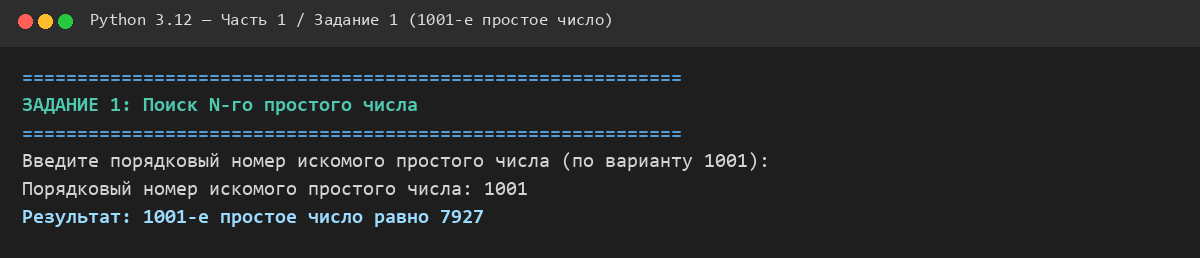
\includegraphics[width=\linewidth, keepaspectratio]{images/fig1_part1_task1.png}
    \caption{Результат выполнения задания 1 (Поиск 1001-го простого числа)}
    \label{fig:p1_t1}
\end{figure}

В результате выполнения оптимизированного алгоритма вычислено, что 1001-м простым числом является число \textbf{7927}.

\begin{figure}[H]
    \centering
    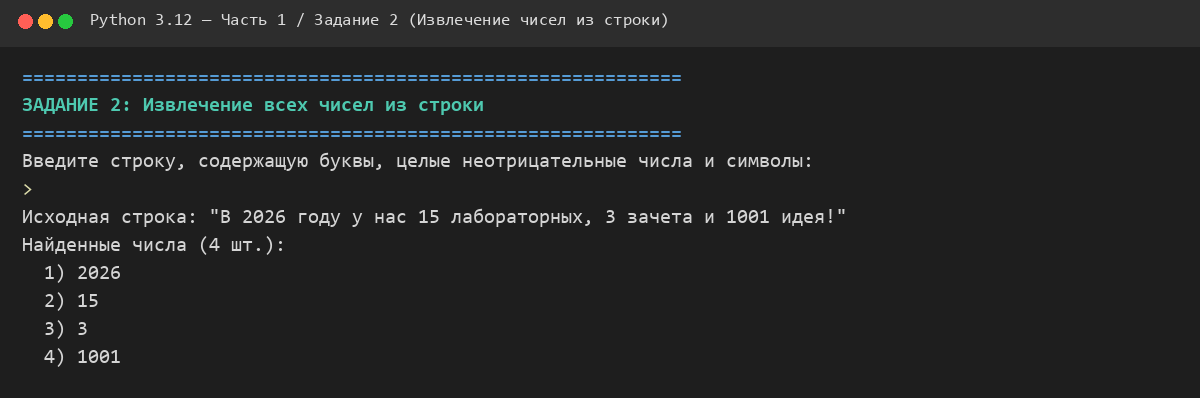
\includegraphics[width=\linewidth, keepaspectratio]{images/fig2_part1_task2.png}
    \caption{Результат выполнения задания 2 (Извлечение чисел из строки)}
    \label{fig:p1_t2}
\end{figure}

Из исходной строки посимвольным разбором успешно извлечены все целые числа: 2026, 15, 3 и 1001.

\begin{figure}[H]
    \centering
    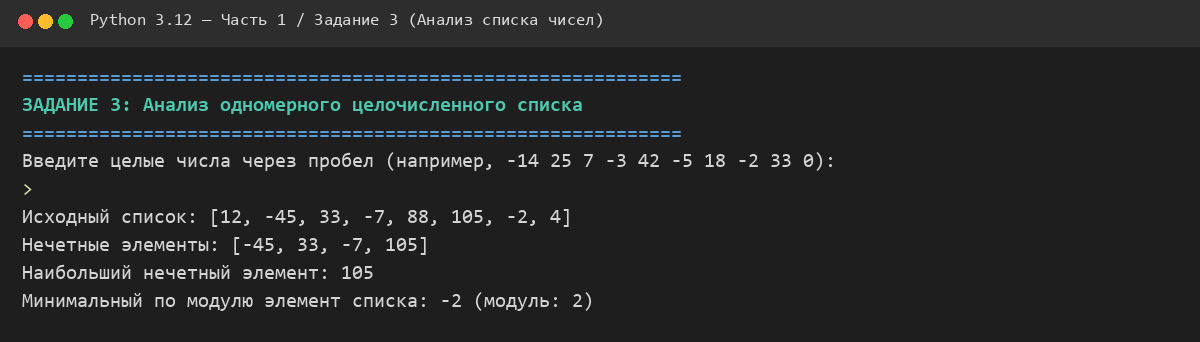
\includegraphics[width=\linewidth, keepaspectratio]{images/fig3_part1_task3.png}
    \caption{Результат выполнения задания 3 (Анализ списка чисел)}
    \label{fig:p1_t3}
\end{figure}

Для введенного списка чисел наибольшим нечетным элементом является \textbf{105}, а минимальным по модулю --- число \textbf{-2}.

\begin{figure}[H]
    \centering
    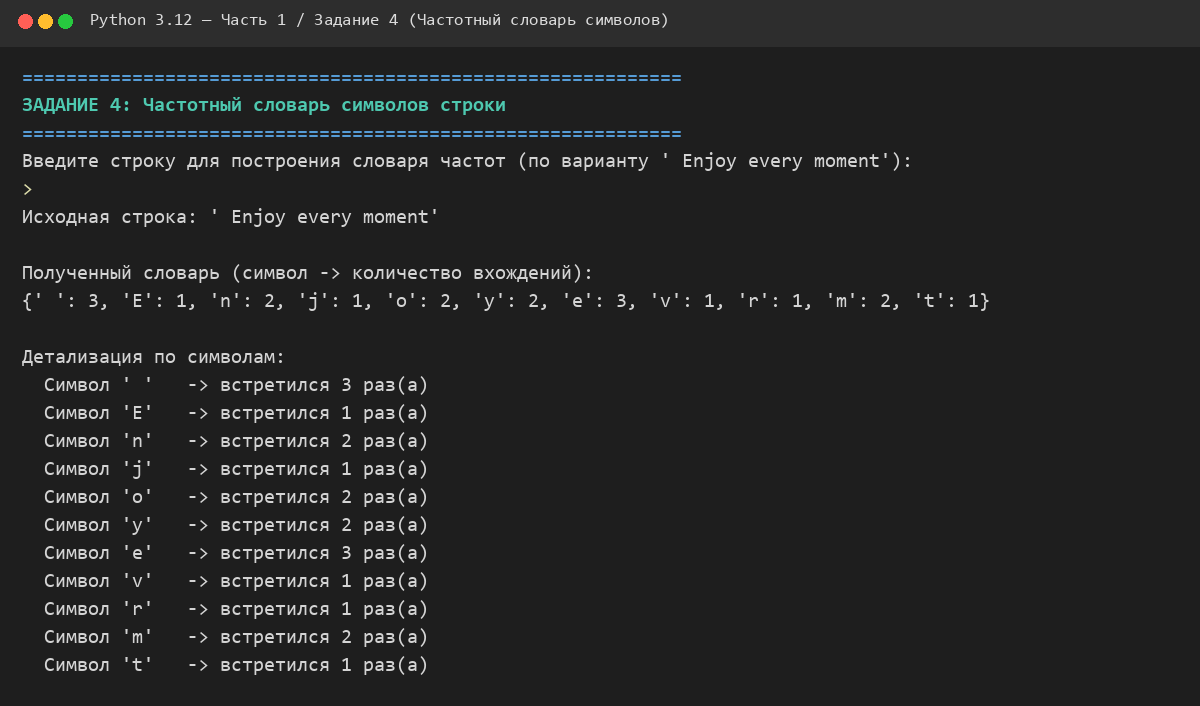
\includegraphics[width=\linewidth, keepaspectratio]{images/fig4_part1_task4.png}
    \caption{Результат выполнения задания 4 (Частотный словарь символов)}
    \label{fig:p1_t4}
\end{figure}

Построена точная частотная таблица вхождений каждого символа исходной строки в виде словаря \texttt{dict}.

\begin{figure}[H]
    \centering
    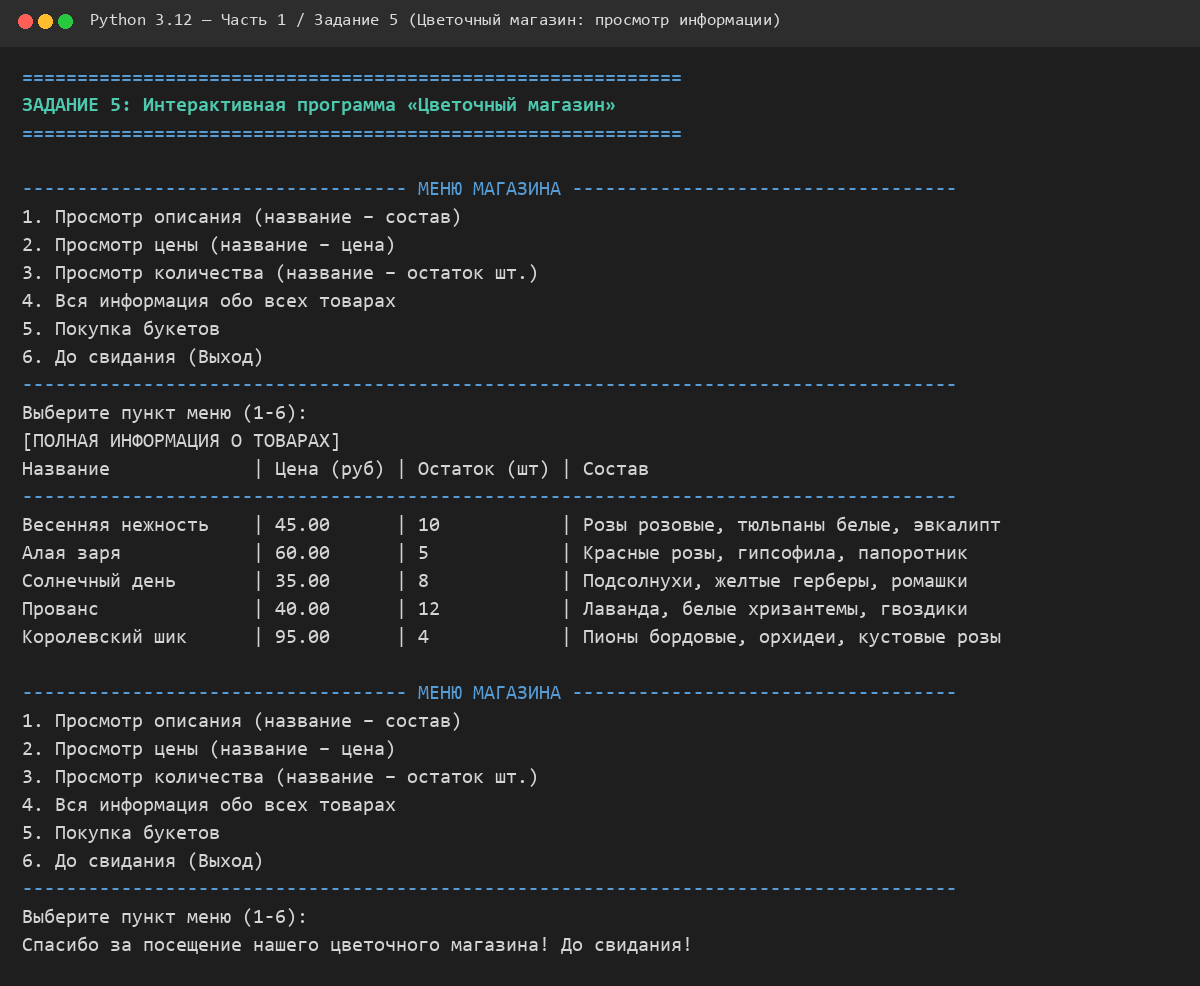
\includegraphics[width=\linewidth, keepaspectratio]{images/fig5a_part1_task5_view.png}
    \caption{Результат выполнения задания 5 (Цветочный магазин: просмотр информации)}
    \label{fig:p1_t5a}
\end{figure}

Продемонстрированы пункты меню просмотра описаний, цен, количества и полной сводной таблицы ассортимента.

\begin{figure}[H]
    \centering
    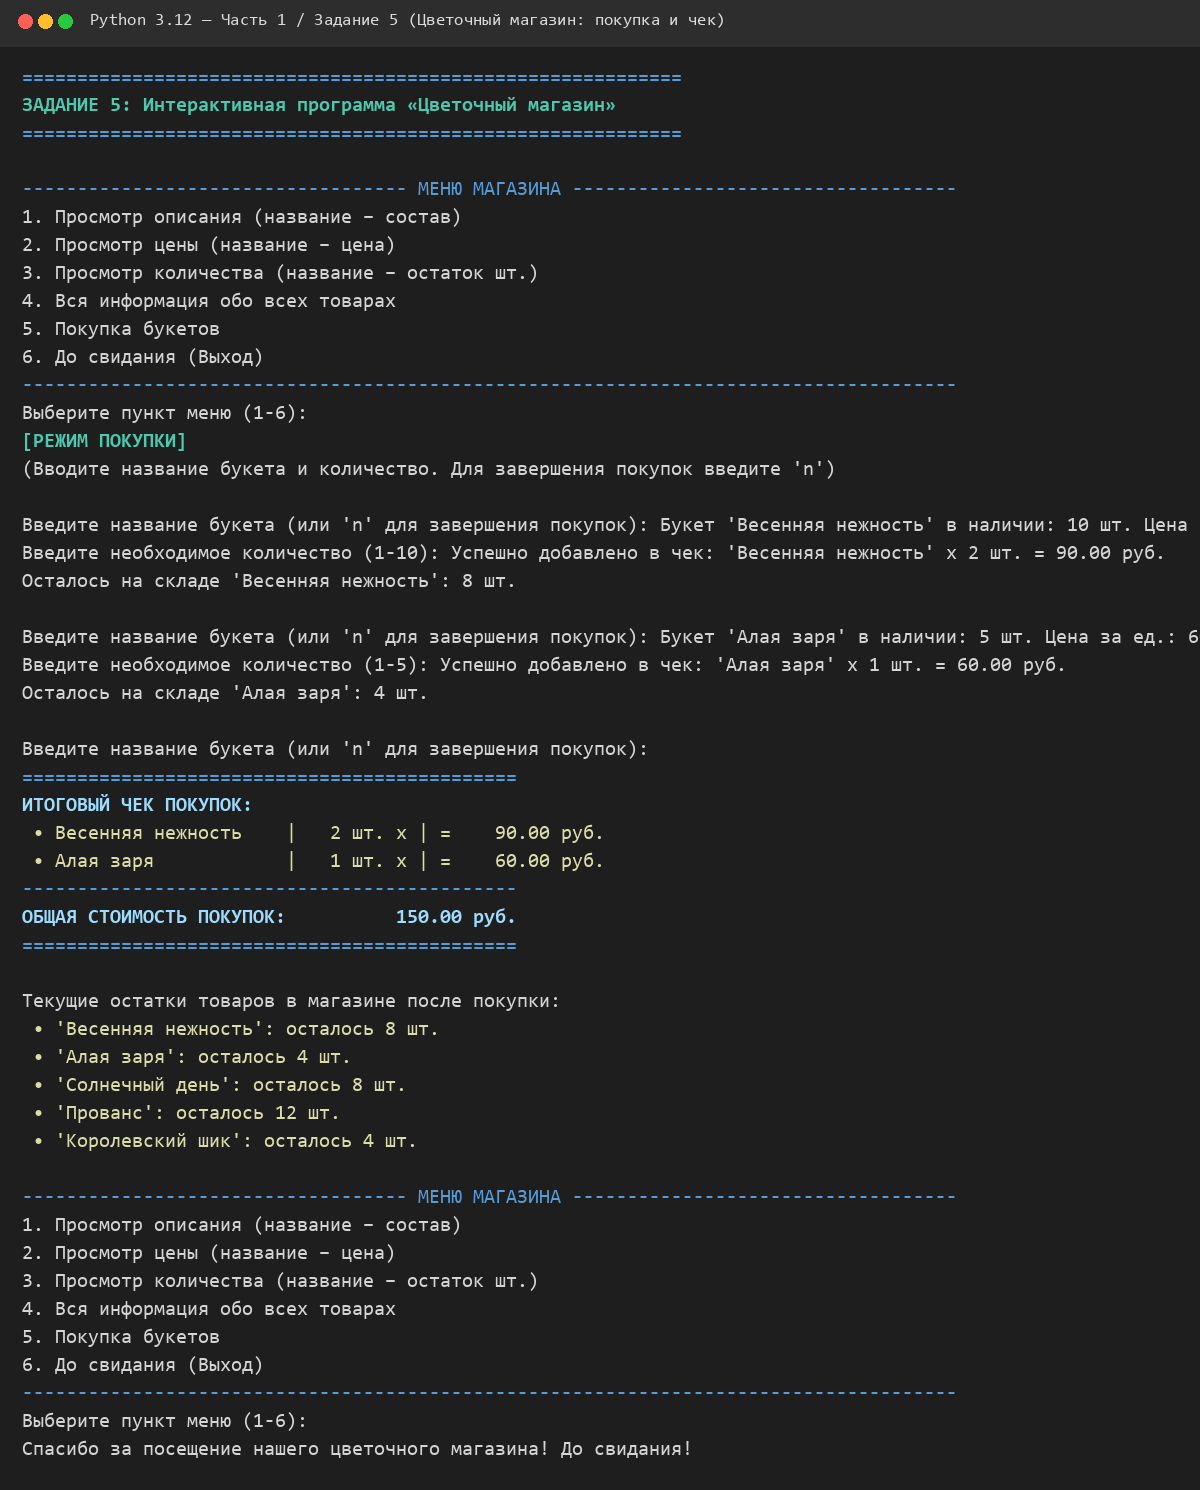
\includegraphics[width=\linewidth, keepaspectratio]{images/fig5b_part1_task5_buy.png}
    \caption{Результат выполнения задания 5 (Цветочный магазин: покупка и чек)}
    \label{fig:p1_t5b}
\end{figure}

Продемонстрирован процесс покупки букетов, автоматический расчет чека (150.00 руб.) и обновление остатков склада.

\begin{figure}[H]
    \centering
    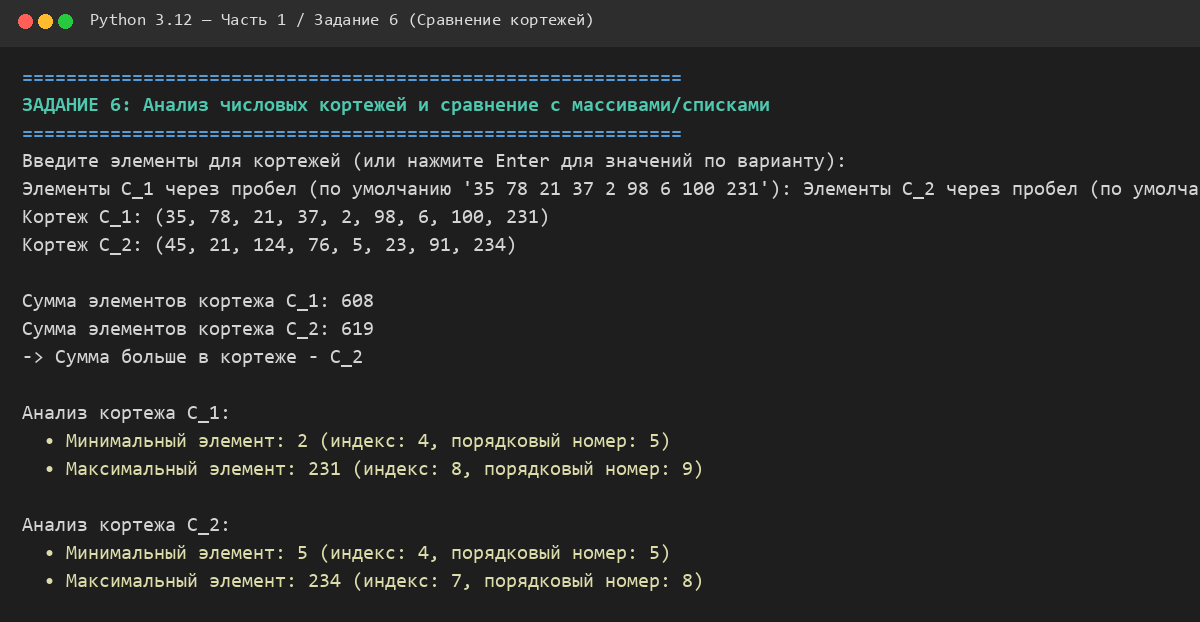
\includegraphics[width=\linewidth, keepaspectratio]{images/fig6_part1_task6.png}
    \caption{Результат выполнения задания 6 (Анализ числовых кортежей)}
    \label{fig:p1_t6}
\end{figure}

Определено, что сумма элементов кортежа $C_2$ (619) превышает сумму $C_1$ (608). Вычислены индексы экстремумов.

\subsection{Результаты выполнения заданий части 2}

\begin{figure}[H]
    \centering
    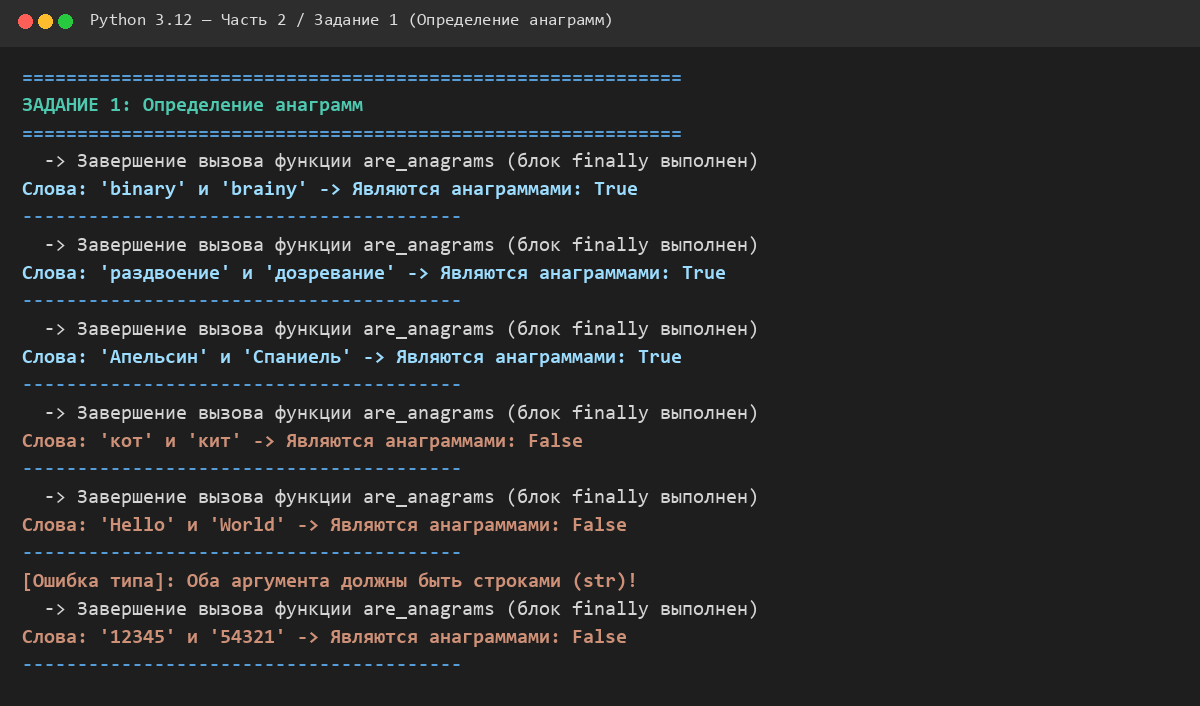
\includegraphics[width=\linewidth, keepaspectratio]{images/fig7_part2_task1.png}
    \caption{Результат выполнения задания 1 (Определение анаграмм)}
    \label{fig:p2_t1}
\end{figure}

Функция корректно верифицирует анаграммы для латиницы и кириллицы, перехватывая ошибки неверных типов.

\begin{figure}[H]
    \centering
    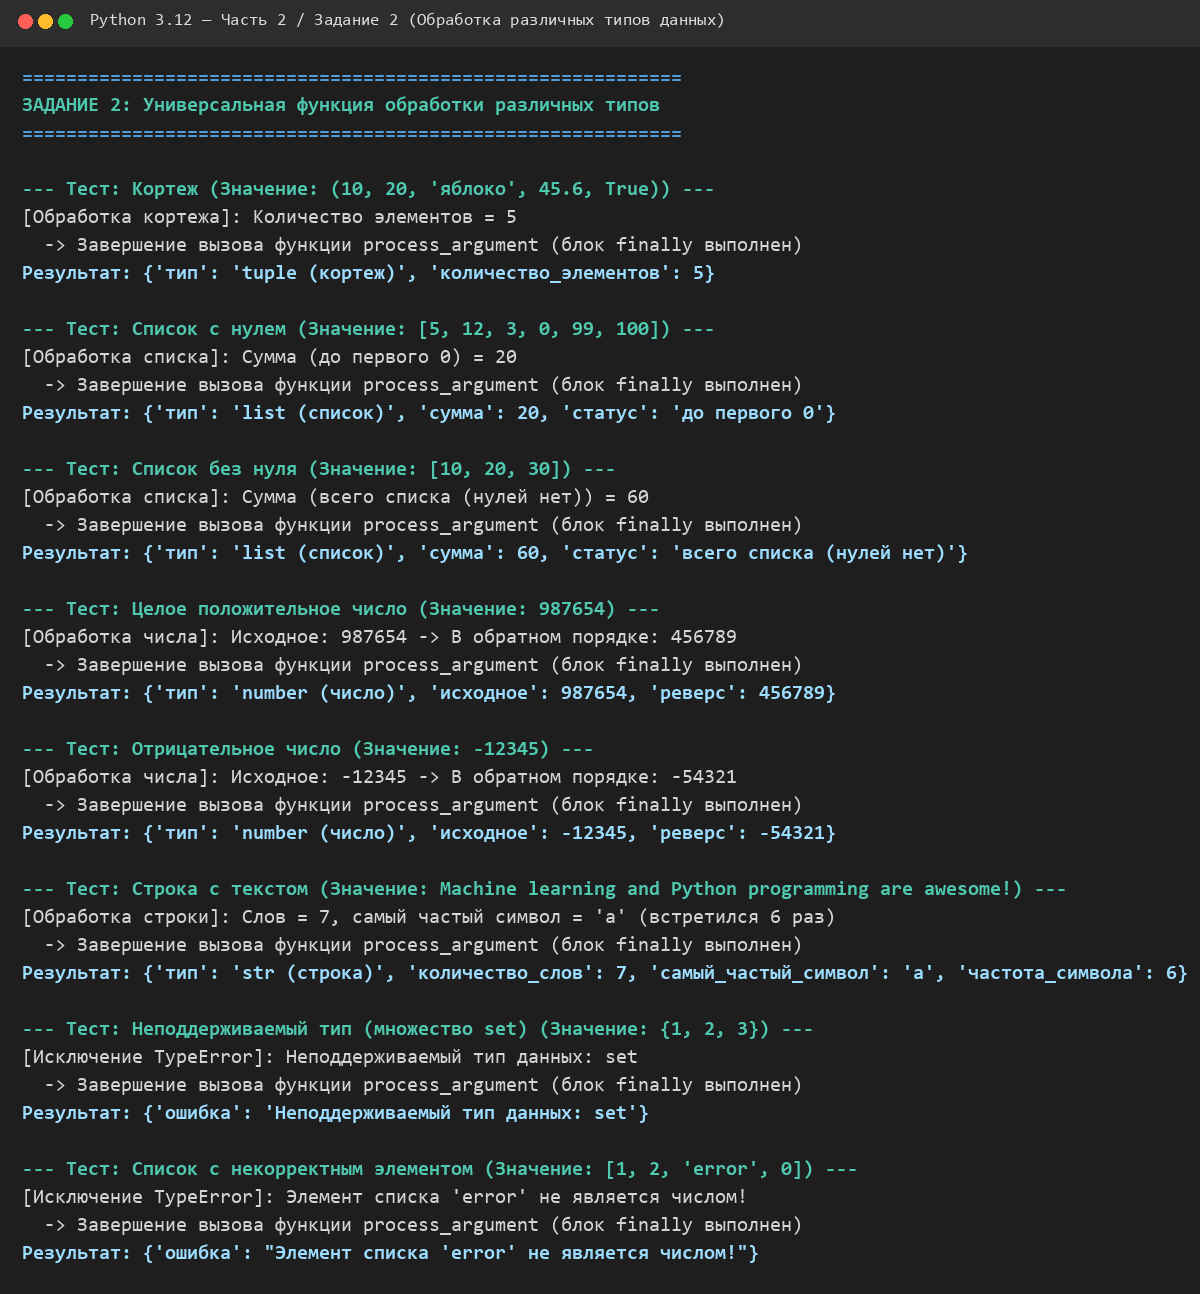
\includegraphics[width=\linewidth, keepaspectratio]{images/fig8_part2_task2.png}
    \caption{Результат выполнения задания 2 (Универсальная обработка типов данных)}
    \label{fig:p2_t2}
\end{figure}

Универсальная функция выполняет вычисления для кортежей, списков (сумма до нуля), чисел (реверс) и строк.

\begin{figure}[H]
    \centering
    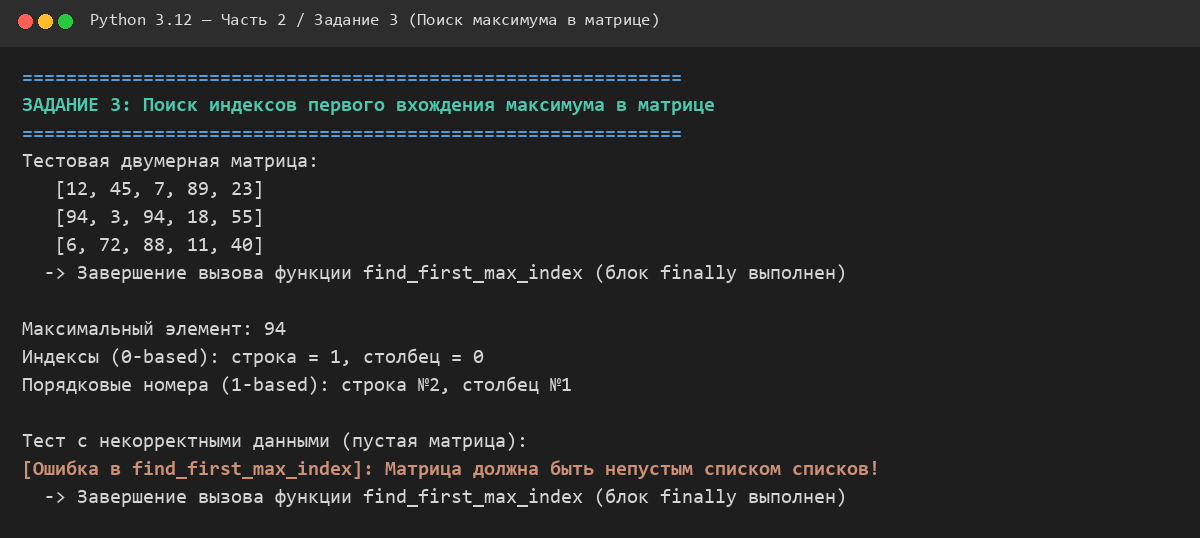
\includegraphics[width=\linewidth, keepaspectratio]{images/fig9_part2_task3.png}
    \caption{Результат выполнения задания 3 (Поиск первого максимума матрицы)}
    \label{fig:p2_t3}
\end{figure}

Для матрицы с дублирующимися максимумами (число 94) функция возвращает индексы первого вхождения (строка №2, столбец №1).

\begin{figure}[H]
    \centering
    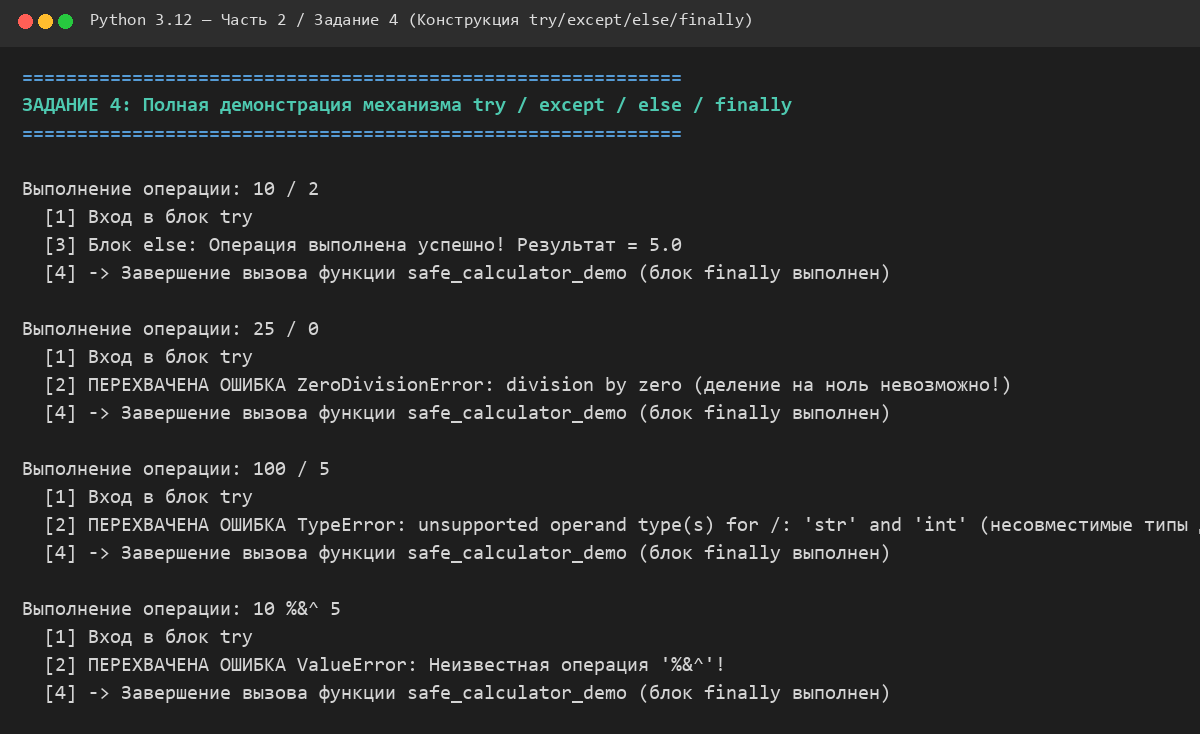
\includegraphics[width=\linewidth, keepaspectratio]{images/fig10_part2_task4.png}
    \caption{Результат выполнения задания 4 (Конструкция try/except/else/finally)}
    \label{fig:p2_t4}
\end{figure}

Наглядно продемонстрирована работа всех четырех секций: штатное завершение, перехват исключений и финализация.

\subsection{Результаты выполнения заданий части 3}

\begin{figure}[H]
    \centering
    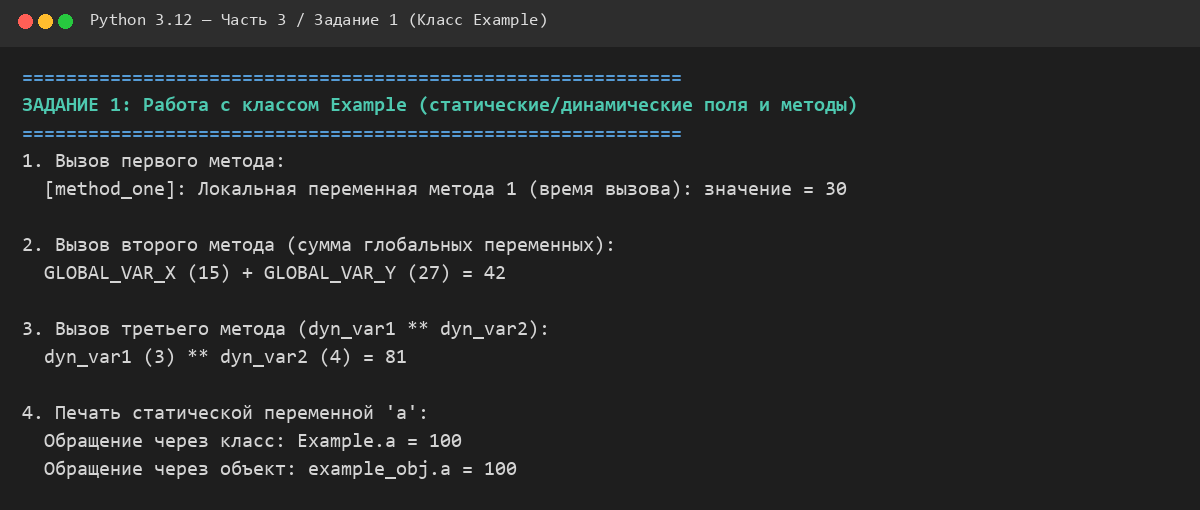
\includegraphics[width=\linewidth, keepaspectratio]{images/fig11_part3_task1.png}
    \caption{Результат выполнения задания 1 (Класс Example)}
    \label{fig:p3_t1}
\end{figure}

Продемонстрирована работа статических и динамических полей класса, доступ к статической переменной \texttt{Example.a}.

\begin{figure}[H]
    \centering
    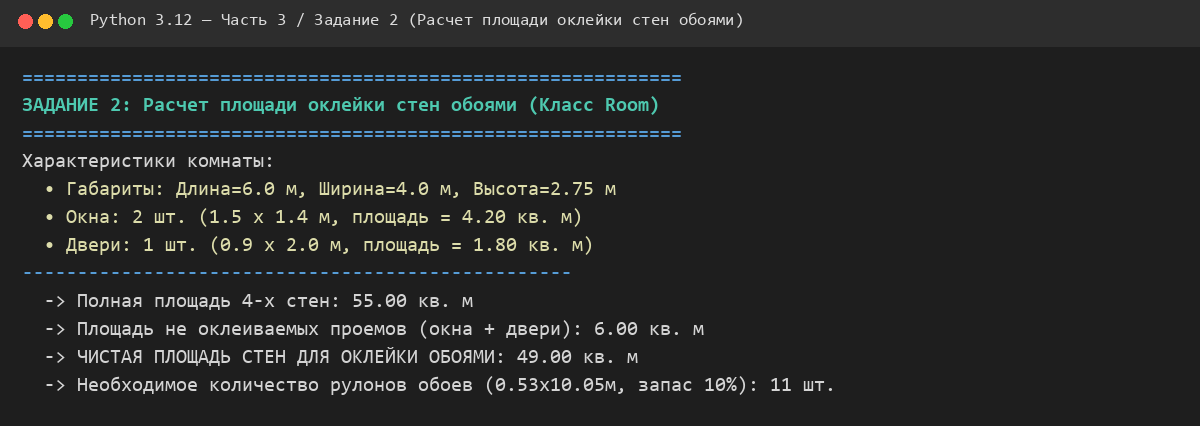
\includegraphics[width=\linewidth, keepaspectratio]{images/fig12_part3_task2.png}
    \caption{Результат выполнения задания 2 (Расчет площади оклейки обоями)}
    \label{fig:p3_t2}
\end{figure}

Вычислена чистая площадь стен комнаты под оклейку обоями (49.00 кв. м) и необходимый объем рулонов (11 шт.).

\begin{figure}[H]
    \centering
    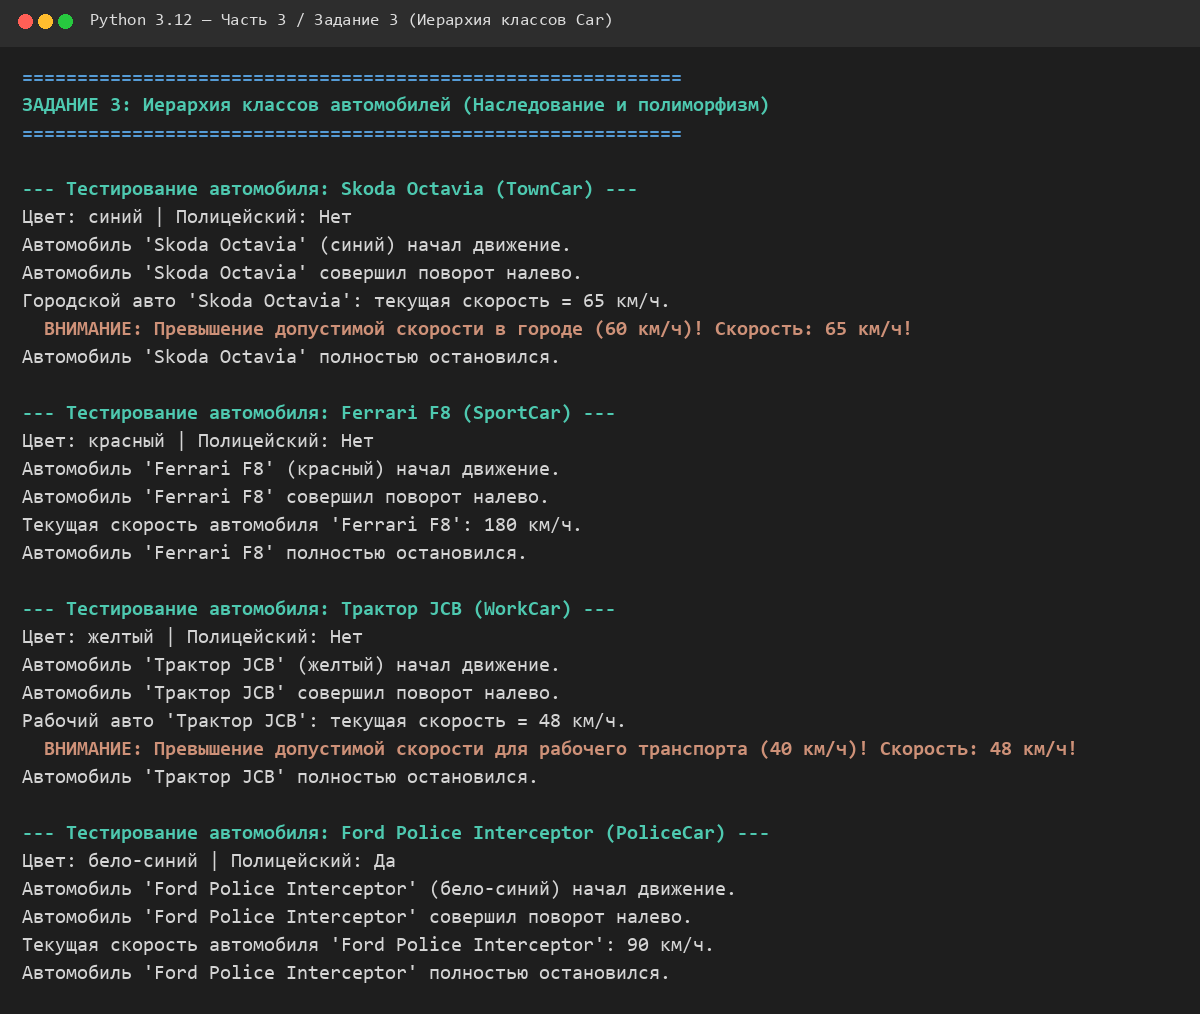
\includegraphics[width=\linewidth, keepaspectratio]{images/fig13_part3_task3.png}
    \caption{Результат выполнения задания 3 (Иерархия классов Car)}
    \label{fig:p3_t3}
\end{figure}

Полиморфизм: переопределенный метод \texttt{show\_speed} выводит предупреждения о превышении скорости для \texttt{TownCar} и \texttt{WorkCar}.

\begin{figure}[H]
    \centering
    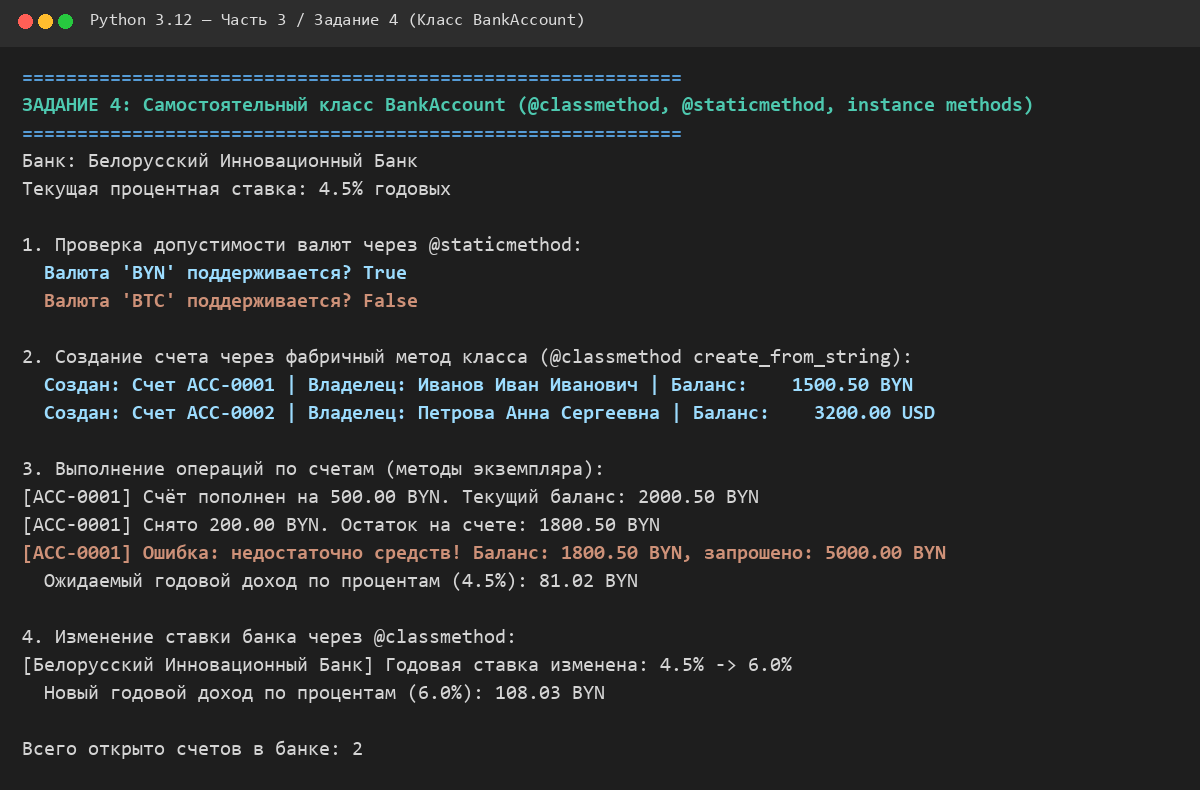
\includegraphics[width=\linewidth, keepaspectratio]{images/fig14_part3_task4.png}
    \caption{Результат выполнения задания 4 (Класс BankAccount)}
    \label{fig:p3_t4}
\end{figure}

Продемонстрирована работа методов экземпляра, фабричного метода \texttt{@classmethod} и статической валидации \texttt{@staticmethod}.

% ==============================================================================
% 6 ВЫВОДЫ ПО ЛАБОРАТОРНОЙ РАБОТЕ
% ==============================================================================
\clearpage
\section{Выводы по лабораторной работе}

В ходе выполнения лабораторной работы №1 по курсу «Методы машинного обучения» были детально исследованы и практически освоены ключевые концепции и инструментарий языка программирования Python 3.12:

\begin{enumerate}
    \item \textbf{По части 1:} Освоен базовый синтаксис языка, динамическая типизация и механизмы работы с коллекциями (\texttt{list}, \texttt{tuple}, \texttt{dict}). Практически подтверждено преимущество неизменяемых кортежей (\texttt{tuple}) в экономии памяти и обеспечении хешируемости по сравнению с изменяемыми списками (\texttt{list}). Разработаны алгоритмы фильтрации простых чисел и посимвольного строкового парсинга.
    \item \textbf{По части 2:} Изучены принципы функциональной декомпозиции и строгой типизации сигнатур функций. Реализована структурная обработка исключительных ситуаций через конструкцию \texttt{try / except / else / finally}, гарантирующая стабильность выполнения программ при некорректных входных параметрах и детерминированное освобождение системных ресурсов.
    \item \textbf{По части 3:} Практически освоена парадигма объектно-ориентированного программирования (ООП). Реализованы прикладные модели с инкапсуляцией геометрических параметров, одиночным наследованием и полиморфизмом методов. Изучены различия областей применения методов экземпляра, фабричных методов класса (\texttt{@classmethod}) и статических методов (\texttt{@staticmethod}).
\end{enumerate}

\end{document}
